\documentclass[12pt]{article}
\title{Information Security Handbook}
\author{David Bailey}
\date{\today}
\usepackage[utf8]{inputenc}
\usepackage[hyphens]{url}
\usepackage{hyperref}
\usepackage{mdframed}
\usepackage{amsmath}
\usepackage{tabularx}
\usepackage{multirow} 
\usepackage{rotating}
\usepackage{lscape}
\usepackage{imakeidx}
\usepackage{tikz}

\indexsetup{level=\section}
\makeindex[name=TC,title=List of Threats and Controls,columns=1,noautomatic]
\makeindex[name=A,title=List of Network Security Assessment Items,columns=1,noautomatic]
\makeindex[name=D,title=List of Documentation Items,columns=1,noautomatic]
\newcommand{\tcitem}[2]{#1 & #2\\}
\newcommand{\tccite}[2]{\index[TC]{#1 -- #2}}
\newcommand{\aitem}[1]{\item #1 \index[A]{#1}}
\newcommand{\ditem}[1]{\item #1 \index[D]{#1}}
\newcommand{\resourcecite}[1]{\hyperref[itm:Resource:#1]{\textsuperscript{\ref{itm:Resource:#1}}}}
\newcommand{\resource}[3][null]{\item #2\\\url{#3}\label{itm:Resource:#1}}

\begin{document}
\maketitle
\newpage
\section*{License}
This work is licensed under the Creative Commons Attribution-ShareAlike 4.0 International License.\\\\To view a copy of the license, visit \url{http://creativecommons.org/licenses/by-sa/4.0/}.
\newpage
\tableofcontents
\newpage
\section{Your First Day}\label{sec:"Your First Day"}
It's your first day as Information Security Officer\resourcecite{WCISO}: everything is broken, servers are hacked, backups are failing, policies are missing, but somehow business goes on. Patients are still being treated. Financial transactions are still being processed. Take a deep breath. If security was easy, you would not have a job. You can make a difference. It will take time.\\\\The primary job of any information security personnel is to reduce risk; however, we often forget about this when we are lost in the details of a critical issue. This handbook is therefore written with a belief in risk management. You cannot eliminate all risks. If a high-risk issue that can be mitigated for cheap, do it. If you cannot justify the cost of a cool product, do not spend the money.\\\\
Before we get started, let me highlight one key for your program: transparency. Transparency in your program is important. Your leadership, coworkers, and customers all have an interest in your Information Security Program. Some security folks hide behind the auspices of security through obscurity\resourcecite{WSTO} and do not discuss their programs. This hurts their program and their organization. Sharing information about your program within your organization (and sometimes outside your organization) strengthens your program. It helps others know what resources are available to them, the benefits of your program, why they should care about your program, and why they should fund your program. These days large organizations such as Google\resourcecite{GVRPR} and Amazon\resourcecite{AWSSC} share information about their security programs publicly and even pay bounties to those who discover bugs in their software.\\\\
\textbf{Resources}
\begin{enumerate}
\resource[WCISO]{Chief information security officer - Wikipedia}{https://en.wikipedia.org/wiki/Chief_information_security_officer}
\resource[WSTO]{Security through obscurity - Wikipedia}{https://en.wikipedia.org/wiki/Security_through_obscurity}
\resource[GVRPR]{Google Vulnerability Reward Program (VRP) Rules}{https://www.google.com/about/appsecurity/reward-program/}
\resource[AWSSC]{Amazon Web Services (AWS) Security Center}{https://aws.amazon.com/security/}
\resource{Outline of computer security - Wikipedia}{https://en.wikipedia.org/wiki/Outline_of_computer_security}
\end{enumerate}
\subsection{Design, Leadership, and Education}
Design, Leadership, and Education are the three most important elements of your Information Security Program. However, these elements are often overlooked in otherwise strong Programs. This is likely because these three are core components of a Masters in Business Administration (MBA); they are not technical. Think of your Information Security Programs as an organization within the organization.\\\\
Design\resourcecite{WDoET} is the most important element of your Program because it is the most effective. Design your Program for everyone in your organization. Consider how every element of your Program interacts with every employee. This includes system administrators, developers, nontechnical coworkers, and you. Also consider those outside your organization. This is an opportunity to start from scratch.\\\\
Think outside the box when you design your Program. I had a great phone call with the Information Security Officer of a Federal organization a couple years ago. He was tired of the state of the industry: "I'm doing everything, I'm following all the best practices, and we still have problems." He was right. Even if you implement everything this handbook recommends, there is still a chance you will be hacked. Sometimes the best approach is to take a step back and redesign your Program from scratch.\\\\
Leadership is the second most important element of your Program. Leadership must believe in your Program and they must support your Program. Your job is to build a program they believe in and support. Support consists of financial resources, human resources, their own compliance with the Program, an email to all employees, etc. Your coworkers need to see support from leadership before they will believe in your Program.\\\\
Education is the third most important element of your Program. First, you need to educate yourself. Educate yourself on your organization: the culture, your coworkers, the policies, and the processes. One of the best ways to do this is with the Assessments. Please see \hyperref[sec:"Assessments, Audits, and Analyses"]{Assessments, Audits, and Analyses} for more information.\\\\
Educate yourself on Information Security. This handbook is a good educational resource, and it contains hundreds of references to other resources. Read books, blogs\resourcecite{KrebsonSecurity}, and websites\resourcecite{DM}\textsuperscript{,}\resourcecite{HackerNews}\textsuperscript{,}\resourcecite{Rnetsec}. Subscribe to mailing lists\resourcecite{USCERTMLF}\textsuperscript{,}\resourcecite{USNISTCSRC}. Watch videos\resourcecite{Lynda}. Listen to podcasts\resourcecite{SpiderLabsRadio}. Join chat rooms\resourcecite{IRCsecurity}. Test new tools. Attend conferences. Take classes\resourcecite{Coursera}\textsuperscript{,}\resourcecite{CourseraCSDomains}\textsuperscript{,}\resourcecite{SANS}. Follow people on Twitter. Join organizations.\resourcecite{ISACA}\textsuperscript{,}\resourcecite{OWASP} Write software. Learn from other organizations in your industry  by looking for at their websites and talking to their Information Security Officers. Educate yourself throughout your career.\\\\
Educate yourself on any laws and regulations that govern your organization. If you work in healthcare, read the HIPAA Security Rule\resourcecite{HIPAASR}. If you accept credit cards, read the Payment Card Industry Data Security Standards\resourcecite{PCIDSS}. These documents are dense and can be hard to read, but you must understand them yourself before you can effectively educate your coworkers. Build you Program with these laws and regulations in mind. 90\% of Information Security is the same in any industry. The 10\% that is different is in these laws and regulations.\\\\
Educate your coworkers.\resourcecite{STH}\textsuperscript{,}\resourcecite{SM} Every employee in your organization needs Information Security education. Design this education so it is appropriate for each employee and effective. Create different education programs for system administrators, developers, and other coworkers. Take everything you have learned about the organization, Information Security, and governing laws and regulations and teach it to your coworkers. Create a catalog of services offered by your Information Security Program.\resourcecite{StanfordIS}\\\\
Educate new employees during their on-boarding. Educate existing coworkers regularly. Educate terminated coworkers during their off-boarding. Please see \hyperref[subsec:"Employee Life Cycle"]{Employee Life Cycle} for more information.\\\\
There are many mediums for education for your employees. Create presentations and speak at meetings and events. Build a website for your Program. Create a library of books. Email newsletters and tips\resourcecite{SANSTips}. Provide tools and services to your organization. Send employees to training and conferences. Create or subscribe to online classes. Recommend mailing lists and websites. Create checklists and "one-pagers." Remember Marketing's Rule of Seven\resourcecite{RuleOf7}: your employees need to hear or see your message seven times before they will buy it. Use many mediums to communicate with your employees.\\\\
Design your education program with Plain Language\resourcecite{PlainLanguage}\textsuperscript{,}\resourcecite{PLAIN}\textsuperscript{,}\resourcecite{PlainEnglishHandbook}. Consider your audience and write for their needs. Clarify complex Information Security concepts, laws and regulations and make them understandable for your audience. Use active voice and positive language. Use simple words and short sentences. Use pictures, bullets, and other design elements to simplify your educational materials. Communicate with your users as they would communicate with themselves. Focus your education on one or two topics at a time. Test your educational materials with a subset of your intended audience. Plain language is one of the most important concepts in a successful program. This paragraph greatly summarizes the importance and implementation of plain language. Remember it is your job to translate complex concepts into understandable education.\\
\begin{mdframed}
\emph{Calvin: I used to hate writing assignments, but now I enjoy them. I realized that the purpose of writing is to inflate weak ideas, obscure poor reasoning, and inhibit clarity. With a little practice, writing can be an intimidating and impenetrable fog!}\\ -- Bill Watterson, Calvin and Hobbes: Homicidal Psycho Jungle Cat
\end{mdframed}\vspace{5mm}
Use Nudge theory\resourcecite{WNudge} to influence your organization's culture. For example, placing the shred bin in front of the trash can makes a difference in where your employees dispose of private information. Make your program visible, open, and honest.\\\\
The Anatomy of an Attack (included as an Appendix) is an example educational presentation. It is brief and suitable for most employees. It covers many high-risk topics and provides guidance for your employees. Customize it for your organization, add a bunch of examples (screenshots), and try it on your employees. Almost every information security company has a piece of marketing with the same title, the Anatomy of an Attack. This presentation is marketing for your Program.\\\\
Everyone is responsible for information security. With Design, Leadership, and Education, you can build information security into your organization's culture and everything your company does. Remember Design is the most effective element in your Program.\\\\
\textbf{Resources}
\begin{enumerate}
\resource[WDoET]{The Design of Everyday Things - Wikipedia}{https://en.wikipedia.org/wiki/The_Design_of_Everyday_Things}
\resource[KrebsonSecurity]{Krebs on Security}{https://krebsonsecurity.com}
\resource[DM]{Daniel Miessler}{https://danielmiessler.com}
\resource[HackerNews]{Hacker News}{https://news.ycombinator.org}
\resource[Rnetsec]{Reddit /r/netsec - Information Security News \& Discussion}{https://reddit.com/r/netsec}
\resource[USCERTMLF]{US-CERT Mailing Lists and Feeds}{https://www.us-cert.gov/mailing-lists-and-feeds}
\resource[USNISTCSRC]{NIST Computer Security Resource Center Mailing List}{https://public.govdelivery.com/accounts/USNISTCSRC/subscriber/new}
\resource[Lynda]{Lynda.com: Online Video Tutorials \& Training}{https://www.lynda.com}
\resource[SpiderLabsRadio]{SpiderLabs Radio}{https://www.trustwave.com/Resources/SpiderLabs-Radio/}
\resource[IRCsecurity]{\#\#security on freenode}{irc://irc.freenode.net/\#\#\#\#security}
\resource[Coursera]{Coursera - Computer Science: Systems \& Security}{https://www.coursera.org/courses?categories=cs-systems}
\resource[CourseraCSDomains]{Coursera - Cybersecurity and Its Ten Domains}{https://www.coursera.org/learn/cyber-security-domain}
\resource[SANS]{SANS}{https://www.sans.org}
\resource[ISACA]{ISACA}{https://www.isaca.org}
\resource[OWASP]{Open Web Application Security Project}{https://www.owasp.org}
\resource[HIPAASR]{HIPAA Security Rule}{http://www.hhs.gov/ocr/privacy/hipaa/administrative/securityrule/securityrulepdf.pdf}
\resource[PCIDSS]{Payment Card Industry (PCI) Data Security Standards (DSS)}{https://www.pcisecuritystandards.org/documents/PA-DSS_v3.pdf}
\resource[STH]{STH.EndUser Security Awareness Training}{https://securingthehuman.sans.org/enduser/}
\resource[SM]{Security Mentor}{https://www.securitymentor.com}
\resource[StanfordIS]{Stanford Information Security}{https://itservices.stanford.edu/security}
\resource[SANSTips]{Security Awareness Tip of The Day}{https://www.sans.org/tip_of_the_day.php}
\resource[RuleOf7]{Your Brand and the Marketing Rule of 7}{http://thewordchef.com/2011/12/your-brand-and-the-marketing-rule-of-7/}
\resource[PlainLanguage]{Plain Language: Improving Communications from the Federal Government to the Public}{http://www.plainlanguage.gov}
\resource[PLAIN]{Plain Language Association International}{http://www.plainlanguagenetwork.org}
\resource[PlainEnglishHandbook]{A Plain English Handbook: How to create clear SEC disclosure documents}{http://www.sec.gov/pdf/handbook.pdf}
\resource[WNudge]{Nudge theory - Wikipedia}{https://en.wikipedia.org/wiki/Nudge_theory}
\end{enumerate}
\subsection{Risk Management}
\begin{mdframed}
\emph{Risk Management: It's Not Rocket Science...It's Much More Complicated}\\ -- John Adams
\end{mdframed}
Risk Management\resourcecite{80039}\textsuperscript{,}\resourcecite{WITRM}\textsuperscript{,}\resourcecite{FISSISRM}\textsuperscript{,}\resourcecite{FAIRWIKI} is Economics, the study of scarcity, applied to Information Security. What is Risk? Like other terms in Information Security, Risk has many definitions. Most people think of risk as...
\begin{equation}
Risk = Something\ Bad\ That\ Can\ Happen
\end{equation}
This is a good definition for informal conversations. However, we need to formalize risk. When we change "Something Bad" to Impact and "Can Happen" to Probability, risk is...
\begin{equation}
Risk = Probability * Impact
\end{equation}
This is a powerful, mathematical definition that we can apply almost anywhere. With this definition, impact can be positive or negative. We can use this definition for decision making by making Pros and Cons lists. Below is an example of the Pros and Cons of increasing required password length from 8 characters to 12 characters.\\\\
\begin{tabularx}{\textwidth}{ X | X }
Pros & Cons\\\hline
Reduced probability of a successful brute-force password attack & Increased probability of users forgetting their passwords\\
 & Increased probability of users writing down their passwords
\end{tabularx}\vspace{5mm}
Here we see that increasing the required password length may not make the system more secure depending on these probabilities. Risk Management balances both sides of a decision. Formal Risk Management programs outside Information Security, such as those that manage financial risk\resourcecite{WFinRisk}, are based on this approach. Consider financial risk and other risks such as employee happiness when making decisions. However, when we add the idea of an threat source exploiting a vulnerability, risk is...
\begin{align}
Risk &= The\ Probability\ a\ Threat\ Source\ Exploits\ a\ Vulnerability \nonumber \\ &\ * The\ Impact\ of\ the\ Vulnerability\ Being\ Exploited
\end{align}
This is the formal definition of Risk for Information Security Programs. NIST SP 800-30 Guide for Conducting Risk Assessments\resourcecite{80030} defines Risk as above with the Risk Model (Figure~\ref{fig:RiskModel}).
\begin{figure}[ht]
\centering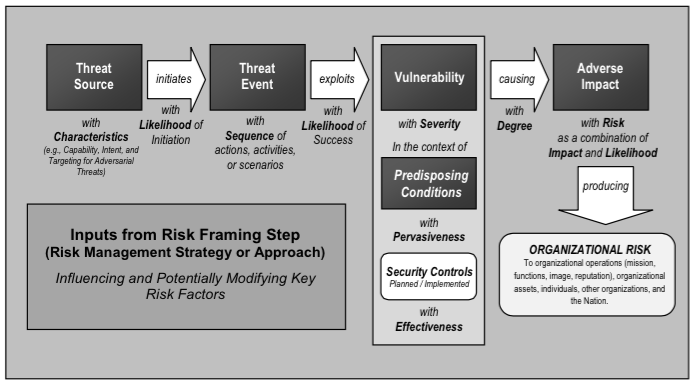
\includegraphics[scale=.55]{./img/RiskModel}
\caption{Risk Model (NIST Special Publication 800-30 Revision 1)}
\end{figure}\label{fig:RiskModel}
The impact of all Information Security risks falls into at least one of three categories:
\begin{itemize}
\item Confidentiality - information can be inappropriately accessed
\item Integrity - information can be inappropriately changed  
\item Availability - information can be made unavailable
\end{itemize}
Confidentiality, Integrity, and Availability are called the CIA triad. Using our example above, you can increase the confidentiality of a system by increasing the required password length, but this can decrease the availability of the system when users forget their passwords. Conversely, you can increase the availability of a system by decreasing the required password length, but this can decrease the confidentiality of the system when attackers successfully brute-force a password. We often forget Integrity in Risk Management, but what good is the information if you can’t trust it to be accurate?\\\\
Using the above definition of risk, NIST SP 800-37 Security and Privacy Controls for Federal Information Systems and Organizations\resourcecite{80037} creates a six step Risk Management Framework\resourcecite{RMFramework} (Figure~\ref{fig:RiskManagementFramework}) that defines a Security Life Cycle for your Information Security Program. Throughout this handbook, we will apply this framework to your organization.
\begin{figure}[ht]
\centering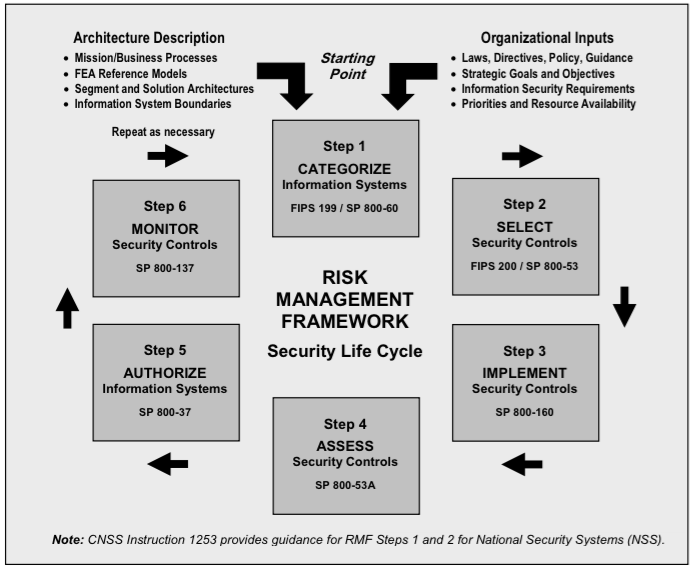
\includegraphics[scale=.55]{./img/RiskManagementFramework}
\caption{Risk Management Framework (NIST Special Publication 800-37 Revision 1)}\label{fig:RiskManagementFramework}
\end{figure}
The steps of the Risk Management Framework are:
\begin{enumerate}
\item Categorize the information system and the information processed, stored, and transmitted by that system based on an impact analysis.
\item Select an initial set of baseline security controls for the information system based on the security categorization; tailoring and supplementing the security control baseline as needed based on an organizational assessment of risk and local conditions.
\item Implement the security controls and describe how the controls are employed within the information system and its environment of operation.
\item Assess the security controls using appropriate assessment procedures to determine the extent to which the controls are implemented correctly, operating as intended, and producing the desired outcome with respect to meeting the security requirements for the system.
\item Authorize information system operation based on a determination of the risk to organizational operations and assets, individuals, other organizations, and the Nation resulting from the operation of the information system and the decision that this risk is acceptable.
\item Monitor the security controls in the information system on an ongoing basis including assessing control effectiveness, documenting changes to the system or its environment of operation, conducting security impact analyses of the associated changes, and reporting the security state of the system to designated organizational officials.
\end{enumerate}
The next section, Information Classification, introduces the concept of categorization. Every section of this handbook contains controls for you to select, implement, assess, and monitor. Chapter 3, Assessments, Audits, and Analyses, details how to assess the security controls you have selected and implemented. Leadership, the second most important element of your Program is responsible for Authorization in your organization.\\\\
Risk management is a powerful tool for your organization because it allows you to formalize and contextualize risk. Use Risk to choose between two projects competing for your time and budget. Use Risk to develop a budget for your Information Security Program. Use Risk to weigh action versus inaction.\\
\begin{mdframed}
"The Goldman Sachs risk system is called SecDB (securities database), and everything at Goldman that matters is run out of it."\resourcecite{SecDB}
\end{mdframed}\vspace{5mm}
\textbf{Resources}
\begin{enumerate}
\resource[80039]{NIST Special Publication 800-39: Managing Information Security Risk - Organization, Mission, and Information System View}{http://csrc.nist.gov/publications/nistpubs/800-39/SP800-39-final.pdf}
\resource[WITRM]{IT Risk Management - Wikipedia}{https://en.wikipedia.org/wiki/IT_risk_management}
\resource[FISSISRM]{Fundamentals of Information Systems Security/Information Security and Risk Management}{https://en.m.wikibooks.org/wiki/Fundamentals_of_Information_Systems_Security/Information_Security_and_Risk_Management}
\resource[FAIRWIKI]{FAIRWIKI: The Definitive Guide to the Factor Analysis of Information Risk (FAIR)}{http://fairwiki.riskmanagementinsight.com}
\resource[WFinRisk]{Financial risk - Wikipedia}{https://en.wikipedia.org/wiki/Financial_risk}
\resource[80030]{NIST Special Publication 800-30 Revision 1: Guide for Conducting Risk Assessments}{http://csrc.nist.gov/publications/nistpubs/800-30-rev1/sp800_30_r1.pdf}
\resource[80037]{NIST Special Publication 800-37 Revision 1: Guide for Applying the Risk Management Framework to Federal Information Systems - A Security Life Cycle Approach}{http://csrc.nist.gov/publications/nistpubs/800-37-rev1/sp800-37-rev1-final.pdf}
\resource[RMFramework]{Risk Management Framework Overview - NIST CSRC}{http://csrc.nist.gov/groups/SMA/fisma/framework.html}
\resource[SecDB]{Why founding a three-person startup with zero revenue is better than working for Goldman Sachs.}{http://blogs.itb.ac.id/djadja/2010/09/15/why-founding-a-three-person-startup-with-zero-revenue-is-better-than-working-for-goldman-sachs-adgrok/}
\end{enumerate}
\subsection{Information Classification}
Information Classification allows us to create different classes of information with different protections. First we will create two different classes of information and then we will determine how to protect those classes.
\begin{description}
\item\textbf{Public Information}\\ Public information is information you would share with everyone. Availability is more important than Confidentiality. In fact, Confidentiality has no importance. Integrity is important. Example availability and integrity risks include a web server that is unavailable or defaced.
\item\textbf{Private Information}\\ Private information is all information that is not public. Other names for this classification include need-to-know, confidential, and proprietary. Confidentiality is more important that Availability. Integrity is important.
\end{description}
This may seem obvious: there is information that we must protect (private) and information that we do not need to protect (public). However, this is the basis of Information Security. Each classification has subclasses specific to your organization. Be clear about what information belongs in each class or subclass. The rest of this handbook describes how we protect these classes of information.\\\\Most laws and regulations use specific data elements to define their classes. HIPAA defines Protected Health Information\resourcecite{WPHI}, PCI defines Account Data, and California SB1386\resourcecite{WSB1386} defines Personally identifiable information\resourcecite{WPII}. Many universities\resourcecite{Harvard}\textsuperscript{,}\resourcecite{CMU}\textsuperscript{,}\resourcecite{Stanford} publish comprehensive data classification matrices. We will talk more about specific laws and regulations in \hyperref[sec:"Policies and Processes"]{Policies and Processes}.\\\\
\textbf{List of Protected Health Information (PHI) Identifiers}\resourcecite{PHI}
\begin{enumerate}
\item Names
\item All geographical identifiers smaller than a state, except for the initial three digits of a zip code if, according to the current publicly available data from the Bureau of the Census: the geographic unit formed by combining all zip codes with the same three initial digits contains more than 20,000 people; and [t]he initial three digits of a zip code for all such geographic units containing 20,000 or fewer people is changed to 000
\item All elements of dates (except year) for dates directly related to an individual, including birth date, admission date, discharge date, date of death; and all ages over 89 and all elements of dates (including year) indicative of such age, except that such ages and elements may be aggregated into a single category of age 90 or older;
\item Phone numbers
\item Fax numbers
\item Email addresses
\item Social Security numbers
\item Medical record numbers
\item Health insurance beneficiary numbers
\item Account numbers
\item Certificate/license numbers
\item Vehicle identifiers and serial numbers, including license plate numbers;
\item Device identifiers and serial numbers;
\item Web Uniform Resource Locators (URLs)
\item Internet Protocol (IP) address numbers
\item Biometric identifiers, including finger, retinal and voice prints
\item Full face photographic images and any comparable images
\item Any other unique identifying number, characteristic, or code except the unique code assigned by the investigator to code the data
\end{enumerate}
\textbf{Table of PCI Identifiers}\resourcecite{PCIDSSI}\\\\
\begin{tabularx}{\textwidth}{| X | X |}
\hline
\multicolumn{2}{| c |}{\textbf{Account Data}} \\
\hline
\textbf{Cardholder Data} & \textbf{Sensitive Authentication Data}\\
\hline
Primary Account Number (PAN) & Full track data (magnetic-stripe\\
Cardholder Name & data or equivalent on a chip)\\
Expiration Date & CAV2/CVC2/CVV2/CID\\
Service Code & PINs/PIN blocks\\
\hline
\end{tabularx}
\\\\\\ 
\textbf{California SB1386}\resourcecite{CASB1386}
\begin{description}
\item(e) For purposes of this section, "personal information" means an individual's first name or first initial and last name in combination with any one or more of the following data elements, when either the name or the data elements are not encrypted: (1) Social security number. (2) Driver's license number or California Identification Card number. (3) Account number, credit or debit card number, in combination with any required security code, access code, or password that would permit access to an individual's financial account. (f) For purposes of this section, "personal information" does not include publicly available information that is lawfully made available to the general public from federal, state, or local government records.
\end{description}
\textbf{Resources}
\begin{enumerate}
\resource[WPHI]{Protected health information - Wikipedia}{https://en.wikipedia.org/wiki/Protected_health_information}
\resource[WSB1386]{California S.B. 1386 - Wikipedia}{https://en.wikipedia.org/wiki/SB_1386}
\resource[WPII]{Personally identifiable information - Wikipedia}{https://en.wikipedia.org/wiki/Personally_identifiable_information}
\resource[Harvard]{Data Classification and Examples (abridged version) - Harvard University}{http://security.harvard.edu/files/it-security-new/files/data_classification_table_abridged_7.23.13_0.pdf}
\resource[CMU]{Guidelines for Data Classification - Carnegie Mellon University}{http://www.cmu.edu/iso/governance/guidelines/data-classification.html}
\resource[Stanford]{Data Classification, Access, Transmittal, and Storage - Stanford University}{http://web.stanford.edu/group/security/securecomputing/dataclass_chart.html}
\resource[PHI]{45 CFR 164.514 - Other requirements relating to uses and disclosures of protected health information.}{http://www.law.cornell.edu/cfr/text/45/164.514}
\resource[PCIDSSI]{Payment Card Industry (PCI) Data Security Standard}{https://www.pcisecuritystandards.org/documents/PCI_DSS_v3.pdf}
\resource[CASB1386]{SB 1386}{http://www.leginfo.ca.gov/pub/01-02/bill/sen/sb_1351-1400/sb_1386_bill_20020926_chaptered.html}
\end{enumerate}
\subsection{Information Inventory and Data Flow Diagrams}
Now that we have defined what information is public and private, we need to inventory it. Ideally we would have an application that automatically tracks every bit of information on every computer within the organization. Some Data Loss Prevention (DLP) software even claims to do this. (Please see \hyperref[subsubsec:"Data Loss Prevention"]{Data Loss Prevention} for more on DLP.) However, there are some more basic approaches. Many organizations use spreadsheets to keep inventories of where information is stored throughout the organization. These can be inflexible and hard to maintain for all but the smallest organizations. I personally prefer data flow diagrams to track information.\\\\
Data flow diagrams\resourcecite{WDFD} are a pictorial representation of where information is created in your organization and where that information travels. They include both storage and transmission of information. Because they can be limited to one type or source of information, they are great for visualizing the entire life of a bit of information. A collection of diagrams can represent all the information in your organization. They are also flexible enough to include arbitrary stores like email, file servers, and printed paper. Last, and most important, data flow diagrams help us  assess risk to data and implement the proper controls to mitigate that risk. Data flow diagrams can be created on whiteboards, paper, or software like Microsoft Visio, Dia, or DOT\resourcecite{WDOT}. A few basic data flows are below.\\\\
\begin{figure}[h]
\centering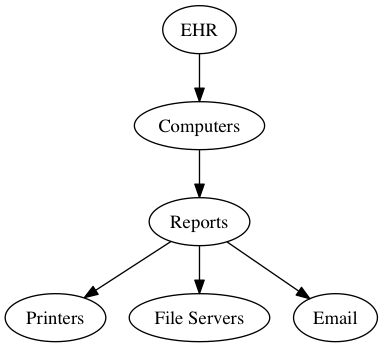
\includegraphics[scale=.75]{./img/ehrDataFlow}
\caption{A basic data flowing showing PHI that originates from the Electronic Health Record (EHR).}
\end{figure}
\begin{figure}[h]
\centering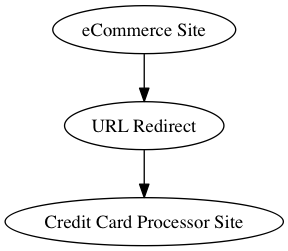
\includegraphics[scale=.75]{./img/eCommerceDataFlow}
\caption{A basic data flow showing credit card information.}
\end{figure}
\newpage
\textbf{Resources}
\begin{enumerate}
\resource[WDFD]{Data flow diagram - Wikipedia}{https://en.wikipedia.org/wiki/Data_flow_diagram}
\resource[WDOT]{DOT (graphic description language) - Wikipedia}{https://en.wikipedia.org/wiki/DOT_(graph_description_language}
\end{enumerate}
\subsection{About this Handbook}
Hopefully you have survived your first day as an Information Security Officer. Read on as we dig into the different areas of Information Security.\\\\
My goal for this handbook is to create an introduction to Information Security and a reference. Please be free to edit sections to better match your organization. Staple in your own organization's documentation for quick reference. Bring this handbook to meetings as a quick reference. Use the appendices to perform your own assessments. Write me (david@davidabailey.com) with your suggestions. Hopefully this book is valuable to everyone from those who are just getting started to Chief Information Security Officers.\\\\
This handbook focuses on the healthcare industry and often uses examples from NIST, HIPAA, and PCI. However, most other regulated industries have similar requirements. The principles of this handbook should apply to all information security programs.\\\\I designed this handbook with vendor neutrality in mind. Vendor selection is often a hostile topic. It is up to your organization to select the vendors and products. The only advise I can give is to disclose and avoid conflicts of interest. There is a lot of BS in the information security world, and it can be hard to make sense of everything. Just remember spending money is not always the best solution, and spending more money is not always better. We tell ourselves we can mitigate all our risk if only we had more money. We get that warm and fuzzy feeling after spending a lot of money. These are false. Money helps, but it is not everything.\\\\
One last thing to remember before we get going is that any or all of you Information Security Program, just like the rest of your business, can be outsourced. It is up to you and your organization to determine when to outsource. Most organizations keep a balance of inside versus outside.\\\\This hand book is structured from high-level to low-level, abstract to concrete, both in terms of information security and organizational structure. Sections build on previous section, but are also designed to be independent. Don't hesitate to jump ahead.\\\\
\textbf{Sections}
\begin{description}
\item \hyperref[sec:"Policies and Processes"]{Policies and Processes}
\item \hyperref[sec:"Assessments, Audits, and Analyses"]{Assessments, Audits, and Analyses}
\item \hyperref[sec:"Networks"]{Networks}
\item \hyperref[sec:"Computers"]{Computers}
\item \hyperref[sec:"Identity and Access Management"]{Identity and Access Management}
\item \hyperref[sec:"Cryptography"]{Cryptography}
\item \hyperref[sec:"Physical"]{Physical}
\end{description}\vspace{5mm}
Each section and subsection of this handbook ends with additional information about the topic where appropriate:
\begin{description}
\item\textbf{Assessment} lists steps for you to evaluate your Information Security Program's effectiveness in this section. This section can be used to build security assessments described in \hyperref[sec:"Assessments, Audits, and Analyses"]{Assessments, Audits, and Analyses}.
\item\textbf{Documentation} lists the relevant documentation your organization needs to address this section. 
\item\textbf{Risk Management} lists the Threats and Controls applicable to this section. This section is a starting point for your risk assessment. 
\item\textbf{Resources} provide additional information about the topics covered in this section. Occasionally there are links to how other organizations are addressing the topic.
\item\textbf{Stories} is a collection of real-life events that highlight risks present in this section. These stories help reiterate the importance of the section to your organization. They are also useful for conveying the importance of your Information Security Program to leadership. Last they provide scenarios for your education program. 
\end{description}
\newpage
\section{Policies and Processes}\label{sec:"Policies and Processes"}
\subsection{Laws, Regulations, and Standards}
In a perfect world, there would be no laws, especially information security laws. Everyone would always do the right thing. However, the world is not perfect and we have laws and regulations that we must follow. Build your Information Security Program around these laws and regulations, not on top of them. If we only follow the letter of the law, our program will be insufficient. Your program should be structured such that it naturally meets the requirements your organization operates within. Always structure your organization to be the least regulated as possible. For example, if you only accept credit cards at two locations, segment those locations from the rest of your network. Last, these laws are usually high-level and leave the details up to you.
\begin{table}[ht]\begin{center}\begin{tabular}{|c|c|c|}\hline
\multirow{12}{.15in}{\begin{turn}{90}Information Security Program\end{turn}} &  &\multirow{6}{.15in}{\begin{turn}{270}Information Security Program\end{turn}} \\
& Laws &\\
& & \\& & \\
& Regulations &\\
& & \\
& Standards & \\
& & \\
& Policies  &\\
& Processes  &\\
& Procedures &\\
& &\\\hline
\end{tabular}\caption{Hierarchy of Governance}\end{center}\end{table}\\
Below is a list of Standards\resourcecite{WCSStandards}, Laws, and Regulations commonly encountered in the United States. All of these programs were created with the same intent: to promote good information secuirty programs. However, there are a few differences highlighted below.
Feel free to skip ahead to Policies if these seem overwhelming.\\\\
\subsubsection{Summary Table of Laws, Regulations, and Standards (Alphabet Soup)}
\begin{table}[ht]\begin{center}\begin{tabular}{ | p{2.5cm} | p{3.5cm} | p{4.5cm} | p{2cm} |}\hline
 & Industry & Sensitive Information & \\\hline
SANS & Any & Any & Guideline\\\hline
ISO & International & Any & Standard\\\hline
NIST & US & Any & Guideline\\\hline
FISMA & Federal government and contractors & Any & Law\\\hline
HIPAA & US Healthcare & EPHI & Law\\\hline
HITRUST & US Healthcare & EPHI & Standard\\\hline
PCI DSS & Credit Cards & Account Data & Regulation\\\hline
GLBA/FFIEC & Finance & Financial Information & Law\\\hline
SSAE & Third-Party Contractors & Any & Standard\\\hline
SOX & Public Companies & Any & Law\\\hline
FERPA & US Education & Student Information & Law\\\hline
NERC & North American Energy & Reliability & Regulation\\\hline
\end{tabular}\end{center}\end{table}
\subsubsection{SANS Critical Security Controls}
The SANS Critical Security Controls\resourcecite{SANSCSC} is a list of the most critical security controls from NIST SP 800-53 (discussed below).The SANS Critical Security Controls is a great place to start any Information Security Program. The list is included as Appendix: SANS Critical Security Controls - Version 5.
\subsubsection{ISO/IEC 27000-series}
ISO/IEC 27000-series\resourcecite{WISO2700} is a family of standards describing how to build and maintain an Information Security Program. It is an international standard. There are numerous modules available, and there is a cost.
\subsubsection{National Institute of Standards and Technology (NIST) Special Publications (SP) 800 Series}
The NIST SP 800 series is a collection of best practice guides for all areas of information security. These guides are the backbone of the federal government's information security programs. Many US and international organizations build their programs around these guides. Many of the concepts of these publications are discussed in this handbook. NIST SP 800-53 Revision 4:  Security and Privacy Controlsfor Federal Information Systems and Organizations\resourcecite{SP80043r4}\textsuperscript{,}\resourcecite{SP80043r4a}\textsuperscript{,}\resourcecite{W80053} is a comprehensive cata-log of security controls for U.S. federal information systems.
\subsubsection{Federal Information Security Management Act of 2002 (FISMA)}
FISMA\resourcecite{NISTFISMAIP}\textsuperscript{,}\resourcecite{WFISMA} is a federal law that requires federal agencies to create an Information Security Program based on the NIST SP 800 Series\resourcecite{NISTSP800} and focuses on the Risk Management Framework described in Risk Management. FISMA requires federal agencies to document\resourcecite{FISMAReporting} all aspects of their Information Security Program. Some federal contracts and grants require FISMA compliance for non-federal organizations. Developing a FISMA program is expensive.
\subsubsection{Health Insurance Portability and Accountability Act (HIPAA) Security Rule}
HIPAA\resourcecite{HIPAASR-P} is a federal law that regulates how Covered Entities (Healthcare Providers, Health Plans, and Health Clearinghouses) and Business Associates store, process, and transmit Electronic Protected Health Information (EPHI). HIPAA (and many other frameworks) divide information security controls into three categories: administrative, physical, and technical. These categories are often defined by the controls in them, and many controls overlap these categories. However, a technical control such as antivirus needs an administrative control to ensure it is properly installed and updated. These categories can often be helpful when framing your program. HIPAA also uses the concept of minimum necessary which is not well defined and somewhat mimics need-to-know\resourcecite{WNeedtoKnow}.
\subsubsection{Health Information Trust Alliance (HITRUST)}
HITRUST\resourcecite{HITRUST}\textsuperscript{,}\resourcecite{WHITRUST} is a three-level, healthcare-specific control framework that cross-references other Information Security Standards to simplify an organization’s compliance requirements. There is a cost.
\subsubsection{Payment Card Industry Data Security Standards (PCI DSS)} 
The PCI DSS\resourcecite{PCIDSS-P}\textsuperscript{,}\resourcecite{PCIKit} is a regulation that applies to anyone accepting credit/debit cards. It focuses on cardhard data including credit/debit card numbers.
\newpage
\begin{table}\begin{center}\begin{tabular}{ | p{5cm} | p{9cm} | }\hline
Control Objectives & PCI DSS Requirements\\\hline
Build and Maintain a Secure Network	& 1. Install and maintain a firewall configuration to protect cardholder data\\
& 2. Do not use vendor-supplied defaults for system passwords and other security parameters\\\hline
Protect Cardholder Data	& 3. Protect stored cardholder data\\
& 4. Encrypt transmission of cardholder data across open, public networks\\\hline
Maintain a Vulnerability Management Program	& 5. Use and regularly update anti-virus software on all systems commonly affected by malware\\
& 6. Develop and maintain secure systems and applications\\\hline
Implement Strong Access Control Measures & 7. Restrict access to cardholder data by business need-to-know\\
& 8. Assign a unique ID to each person with computer access\\
& 9. Restrict physical access to cardholder data\\\hline
Regularly Monitor and Test Networks & 10. Track and monitor all access to network resources and cardholder data\\
& 11. Regularly test security systems and processes\\\hline
Maintain an Information Security Policy	& 12. Maintain a policy that addresses information security\\\hline
\end{tabular}\end{center}\end{table}
\newpage
\subsubsection{Federal Financial Institutions Examination Council (FFIEC) IT Examination Handbooks}
The FFIEC regulates the financial industry through audits against their handbooks\resourcecite{FFIECBooks}. The underlying regulations protect financial information.
\subsubsection{Statement on Standards for Attestation Engagements (SSAE) 16}
SSAE 16 is a financial auditing standard that is performed by Certified Public Accountants (CPAs) against service organizations. It does not replace a Risk Assessment.
\subsubsection{Sarbanes-Oxley Act of 2002 (SOX)}
Sarbanes-Oxley Act of 2002 (SOX)\resourcecite{SOX404}
\subsubsection{Family Education Rights and Privacy Act of 1974 (FERPA; also know as the Buckley Amendment)}
\subsubsection{North American Electric Reliability Corporation (NERC)}
\subsubsection{State Laws}
\textbf{Resources}
\begin{enumerate}
\resource[WCSStandards]{Cyber Security Standards - Wikipedia}{https://en.wikipedia.org/wiki/Cyber_security_standards}
\resource[SANSCSC]{SANS Critical Security Controls}{http://www.sans.org/critical-security-controls/}
\resource[WISO2700]{ISO 27000 Series - Wikipedia}{https://en.wikipedia.org/wiki/ISO/IEC_27000-series}\
\resource[SP80043r4]{NIST Special Publication 800-53 Revision 4: Security and Privacy Controls for Federal Information Systems and Organizations}{http://nvlpubs.nist.gov/nistpubs/SpecialPublications/NIST.SP.800-53r4.pdf}
\resource[SP80043r4a]{NIST Special Publication 800-53A Revision 4: Assessing Security and Privacy Controls in Federal Information Systems and Organizations}{http://nvlpubs.nist.gov/nistpubs/SpecialPublications/NIST.SP.800-53Ar4.pdf}
\resource[W80053]{NIST Special Publication 800-53 - Wikipedia}{https://en.wikipedia.org/wiki/NIST_Special_Publication_800-53}
\resource[NISTFISMAIP]{NIST FISMA Implementation Project}{http://csrc.nist.gov/groups/SMA/fisma/index.html}
\resource[WFISMA]{Federal Information Security Management Act of 2002}{https://en.wikipedia.org/wiki/Federal_Information_Security_Management_Act_of_2002}
\resource[NISTSP800]{NIST Special Publications 800 Series}{http://csrc.nist.gov/publications/PubsSPs.html}
\resource[FISMAReporting]{FY 2010 Reporting Instructions for the Federal Information Security Management Act and Agency Privacy Management}{http://www.whitehouse.gov/sites/default/files/omb/assets/memoranda_2010/m10-15.pdf}
\resource[HIPAASR-P]{HIPAA Security Rule}{http://www.nist.gov/healthcare/security/hipaasecurity.cfm}
\resource[WNeedtoKnow]{Need to know - Wikipedia}{https://en.wikipedia.org/wiki/Need_to_know}
\resource[HITRUST]{HITRUST Alliance}{http://hitrustalliance.net}
\resource[WHITRUST]{HITRUST - Wikipedia}{https://en.wikipedia.org/wiki/HITRUST}
\resource[PCIDSS-P]{PCI DSS}{https://www.pcisecuritystandards.org/documents/PCI_DSS_v3.pdf}
\resource[PCIKit]{Open PCI Scoping Toolkit}{http://itrevolution.com/wp-content/uploads/2012/08/OpenPCIScopingToolkit.pdf}
\resource[FFIECBooks]{FFIEC IT Examination Handbook}{http://ithandbook.ffiec.gov/it-booklets.aspx}
\resource[SOX404]{SOX 404 top–down risk assessment - Wikipedia}{https://en.wikipedia.org/wiki/SOX_404_top–down_risk_assessment}
\end{enumerate}
\subsection{Policies}
Policies are the highest level of control at your organization. They help align your organization to applicable laws and regulations. Polices protect your organization, your employees, and your customers.\\\\
Because policies are created out of nothing, they require strong employee buy-in from all levels to be successful. Policy creation should involve all parts of the organization from top down and across all departments. Leadership must believe in your organization's policies, follow them, and enforce them fairly across the entire organization. This builds a strong foundation for your Information Security Program. Your policies, combined with the laws and regulations applicable to your industry, help your organization run legally and efficiently. Make vendors aware of your policies when applicable.\\\\
Policies must list consequences for non-compliance\resourcecite{WShadowIT}. Terms such as can, should, shall, and must need to be properly defined\resourcecite{RFC2119} and understood. If an employee can or should do something, does the employee have to do it?\\\\
If you need to create policies, start by documenting existing unwritten policies and processes. Many organizations download policies from SANS\resourcecite{SANSPolicies} or other organizations\resourcecite{catalyze}, change the company name, and claim they have policies. This does nothing but maybe fool an auditor. No one understands these policies or follows them. Policies templates can be useful as guides, but write your own policies that reflect your organization.\\\\
We will discuss specific policies throughout the remainder of this section and throughout this book. However, it is important to remember that policies hold the most legal strength in your organization. Employees can be fired and contracts can be terminated because of policy violations. Remember to use Plain Language when writing your policies. Review the paragraph on Plain Language in Design, Leadership, and Education and read some of the Resources in that section. To borrow terms from Creative Commons, if you write your policies in Legal English, make sure there is also a human-readable copy. For example, the SANS Dial-In Access Policy states "It is the responsibility of employees with dial-in access privileges to ensure a dial-in connection to \textless Company Name\textgreater  is not used by non-employees to gain access to company information system resources." This could also be written "Don't share your dial-in credentials." The rewritten version is shorter and clearer. This makes it more likely to be followed. However, I also wonder if anyone uses dial-up these days...
\subsection{Acceptable Use Policy}
An Acceptable Use Policy\resourcecite{WAUP}\textsuperscript{,}\resourcecite{PennAUP} clearly states the who, what, why, when, and how employees can and cannot use your organization's network and computers. This document, like all policies makes sure the employee and the organization understand the rules. All organizations need an Acceptable Use Policy.
\subsection{Information Security Policy}
Information Security Policies\resourcecite{HarvardISP}\textsuperscript{,}\resourcecite{BerkeleyMSSND} provide additional requirements for how employees use information and computers. These policies can be combined into one document or separated into several documents based on topics. Below are the most common topics covered in Information Security Policies with links to the relevant section of this book.
\subsubsection{Information Classification}
\subsubsection{Information Retention and Destruction}
\subsubsection{Change Management}
\subsubsection{Vendors}
\subsubsection{Incident Reporting and Incident Response}
\subsubsection{Disaster Recovery and Business Continuity Planning}
\subsubsection{Vulnerability Assessment and Management}
\subsubsection{Networks: Firewalls, Wireless, Remote Access}
\subsubsection{Computers: Central Management, Anti-Malware, Host-Based Firewall, Backups, etc.}
\subsubsection{Mobile Devices: Laptops, Smartphones, Mobile drives, etc.}
\subsubsection{Email, Phones, Faxes, Instant Messaging, etc.}
\subsubsection{Logs and Monitoring}
\subsubsection{Access Control: Accounts and Passwords}
\subsubsection{Encryption}
\subsubsection{Visitors}
\textbf{Resources}
\begin{enumerate}
\resource[WShadowIT]{Shadow IT - Wikipedia}{https://en.wikipedia.org/wiki/Shadow_IT}
\resource[SANSPolicies]{SANS - Information Security Policy Templates}{https://www.sans.org/security-resources/policies/}
\resource[catalyze]{Catalyze - Company Policies for HIPAA Compliance}{http://catalyzeio.github.io/policies/}
\resource[RFC2119]{RFC 2119 - Key words for use in RFCs to Indicate Requirement Levels}{http://tools.ietf.org/html/rfc2119}
\resource[WAUP]{Acceptable Use Policy - Wikipedia}{https://en.wikipedia.org/wiki/Acceptable_use_policy}
\resource[PennAUP]{Penn Computing: Policy on Acceptable Use of Electronic Resources}{http://www.upenn.edu/computing/policy/aup.html}
\resource[HarvardISP]{Harvard University - Information Security Policy}{http://policy.security.harvard.edu}
\resource[BerkeleyMSSND]{UC Berkeley - Minimum Security Standards for Networked Devices (MSSND)}{https://security.berkeley.edu/MinStds/AppA.min.htm}
\resource{An Overview of the Organizational Guidelines}{http://www.ussc.gov/sites/default/files/pdf/training/organizational-guidelines/ORGOVERVIEW.pdf}
\end{enumerate}
\subsection{Processes (and Procedures, and Standards, and Guidelines)}
Processes, Procedures, Standards, and Guidelines provide structure to your Information Security Program and help to standardize work.
\subsection{Life Cycles}\label{subsubsec:"Computer Lifecycle"}
People have a life cycle: birth, childhood, adulthood, and death. Information also has a life cycle. Networks, computers, applications, employees, and vendors have a life cycle. A generic life cycle is:
\begin{enumerate}
\item Proposal
\item Review
\item Approve
\item Implement
\item Maintain
\item Sunset
\end{enumerate}
In other words, buy something, set it up, use it, and get rid of it. The details of this process is different at each organization, but the key elements are the same.\\\\
Integrate your Information Security Program into the appropriate steps of your organization's life cycles. Consult the business owner during the proposal. Conduct an assessment including a risk assessment and a questionnaire during the review. Also classification information. Require leadership approval before implementation. Run your computer hardening process or network device hardening process during implementation. These are discussed later in this section. Also, add the item to your applicable inventory. Conduct periodic assessments as maintenance. Properly dispose of items during sunsetting.\\\\
Document your organization's life cycles and educate your employees on your organization's life cycles.
\subsection{Employee Life Cycle}\label{subsec:"Employee Life Cycle"}
There are many different job roles with different interests that interact with information security. For example, at a hospital we have
\begin{itemize}
\item Doctors and nurses who provide care for patients. They are heavy users of information,
\item Information Technology who enables the hospital to operate. They like to do cool things with fun toys,
\item Finance and administration who try to reduce cost,
\item Lawyers who reduce legal liability at the hospital,
\item And many other job roles with their own interests.
\end{itemize}
All these interests are often in conflict with each other. We sometimes call these conflicts politics or bureaucracy. However, they can all be calculated with risk.\\\\
People are your organization's most important information security control. All your employees are critical to protecting your information from attackers. Employees use information security controls all day, every day. They are also blamed for breaches. However, each failure of an employee protecting information is a failure of your information security program. Did your program educate the employee peoperly? Did your organization provide the employee with the proper resources? Evaluate the roles of employees within the context of an employee life cycle: 
\begin{itemize}
\item Onboarding
\item Ongoing
\item Offboarding
\end{itemize} We are using the term employee, but these concepts apply to anyone who works in or for your organization including contractors, volunteers, temporary staff, etc.
\subsubsection{Onboarding}
The onboarding process is everything from creating a job requisition through an employee's initial training. Begin by including including information security in job descriptions where appropriate. Consider requiring and paying for security certifications for certain positions. Everyone from information security analysts to receptions to janitors has a responsibility for information security. Make sure you hire people who have the proper experience and understand security. Ask about information security concepts during job interviews.\\\\
Many industries require various background checks (criminal, civil, and other) and reference checks. In other industries, these are a good idea. Other organizations shy away from these checks. Implement the appropriate checks for your organization and industry.\\\\
Introduce your Information Security Program to all employees at orientation. This is the beginning of your education program for each employee. Continue educating employees at orientation and throughout their employment.
Some organizations ask their coworkers to complete an attestation if they have access to sensitive information or not. If they do not work with sensitive information, they may be able to forgo the some of the requirements of your security program.
\subsubsection{Ongoing}
A great start goes a long way for introducing your employees to your information security program and company culture. However, you also need constant reinforcement. Continue your education program with periodic (weekly, monthly, yearly, etc.) education.
\subsubsection{Offboarding}
The offboarding process is the conclusion of the employee life cycle. Employees leave organizations voluntarily and involuntarily. The offboarding process should for both situations must contain the same elements in both situations. Remind the employee of his or her responsibilities and retrieve information that is the property of the organization from the employee.
\subsection{Vendor Life Cycle}
Vendors, contractors, service providers, business associates. Whatever you call them, these organizations contract with your organization to perform a service. Anytime you provide your information or access to your information to an outside organization your must perform due diligence. Due diligence means you evaluate the risks of doing business with the outside organization and mitigate those risks. We will look at the vendor life cycle similar to the employee life cycle: contracting, ongoing due diligence, and contract termination.\\\\
Everyone is excited about Cloud Computing (Infrastructure as a Service, Platform as a Service, and Software as a Service). However, Cloud Computing is nothing new to  information security. We have been contracting with these services for decades.
\subsubsection{Contracting}
Follow your purchasing process and have your purchasing, legal, risk management, intellectual property, etc. departments review the contract. Many organizations add specific language to any contract where the vendor will have access to sensitive information. These requirements could include conditions for access to the information, acceptable locations for access and storage of information (i.e. no offshoring), requirements for notifications of a breach, requirements for deletion of information when the contract is terminated, etc. Again, your purchasing and/or legal departments should help you with contracts.\\\\
Conduct an assessment of each vendor before signing a contract. This assessment could be as simple as a short questionnaire, or it could involve all the topics covered under Assessments. Several example questionnaires are included in Resources. Some vendors have prepared answers for standard questionnaires.\\\\
Some organizations require vendor's employees who will have access to sensitive information to sign the organization's acceptable use policy or a specially created document. Again, ask for this before the contract is signed.\\\\
Many organizations will often make claims such as HIPAA-compliant or SAS-70 compliant. These are not a substitute for your due diligence. FedRamp is an interesting new federal program where one federal department can sponsor the due diligence effort for a vendor and then other departments can use that same effort. This will hopefully reduce some of the duplication required for government contracts.
Please see \hyperref[subsubsec:"Business Associate Agreements"]{Business Associate Agreements} below for specific requirements in the healthcare industry.
Vendor Questionnaire organized the same as this book. Go through the Table of Contents and think about the questions that you want to ask the vendor. All organizations are different and will ask different questions. Many vendors have prepared statements about their Information Security controls that could be used in place of a questionnaire. May have one questionnaire for all vendors. May have different questionnaires for externally-hosted application, internally-hosted application, other, etc.
\subsubsection{Business Associate Agreements}\label{subsubsec:"Business Associate Agreements"}
If you work at a healthcare organization, you should be familiar with business associate agreements. These agreements must be in place with any business associates. If you are not a healthcare organization, ignore this section.
\subsubsection{Ongoing Due Diligence}
Once your organization and the vendor have singed a contract, you must continue your due diligence. Periodically reassess each vendor.
\subsubsection{Contract termination}
Similar to when you terminate an employer-employee relationship, make sure the terms of the contract are followed when you terminate it. If the contract states the vendor must delete all copies of your data, verify this has happened.\\\\
\textbf{Assessment}
\begin{description}
\item Verify you have a signed Business Associate Agreement on file for all Business Associates.
\end{description}
\textbf{Documentation}
\begin{description}
\ditem{Business Associate Agreement}
\ditem{Business Associate Policy}
\end{description}
\textbf{Risk Management}\\\\
\begin{tabularx}{\textwidth}{ X | X }
Threats & Controls \\
\hline
\tcitem{Information Security Risk at a Business Associate}{Business Associate Agreement}
\end{tabularx}\vspace{5mm}
\tccite{Information Security Risk at a Business Associate}{Business Associate Agreement}
\textbf{Resources}
\begin{enumerate}
\resource[]{Practical Measurement Framework for Software Assurance and Information Security}{https://buildsecurityin.us-cert.gov/sites/default/files/SwA_Measurement.pdf}
\resource[]{ISO 27002 Security Benchmark}{https://nigesecurityguy.wordpress.com/2013/05/28/iso-27002-security-benchmark/}
\resource[]{Information Security Program Assessment Tool}{http://www.educause.edu/library/resources/information-security-program-assessment-tool}
\resource[]{Information Security Risk Assessment Checklist}{http://www.cio.ca.gov/OIS/Government/documents/docs/RA_Checklist.doc}
\resource[]{CSA Security, Trust \& Assurance Registry}{https://cloudsecurityalliance.org/star/}
\resource[]{Consensus Assessments Initiative Questionnaire v3.0.1}{https://cloudsecurityalliance.org/download/consensus-assessments-initiative-questionnaire-v3-0-1/}
\resource[]{Business Associate Contracts}{http://www.hhs.gov/ocr/privacy/hipaa/understanding/coveredentities/contractprov.html}
\end{enumerate}
\subsection{Inventories}
Inventory document information and where it processed, stored, and transmitted.
\subsubsection{Information}
Use Data Flow Diagrams, discussed in Your First Day, to help inventory your information. Some Data Loss Prevention (DLP) products claim to inventory all your information.
\subsubsection{Networks and Computers}
Inventory your networks, network devices, and computers. Use directory services (Active Directory), DNS, and DHCP to keep records. Scan the network to verify your inventories. Optionally, keep manual inventories. Ensure inventories are up-to-date.
\subsubsection{Media}
\subsubsection{Applications}
\subsubsection{Vendors}
\textbf{Resources}
\begin{enumerate}
\resource{Visa Global Registry of Service Provider}{http://www.visa.com/splisting/searchGrsp.do}
\end{enumerate}
\subsubsection{Inventory Examples}
\begin{landscape}
\begin{table}[h]\begin{center}\begin{tabular}{|l|l|l|l|l|l|l|l|}\multicolumn{8}{l}{\textbf{Computer Inventory}}\\\hline
\parbox[t]{1cm}{Employee} & \parbox[t]{2.5cm}{Type} & \parbox[t]{1cm}{Model} & \parbox[t]{3cm}{Serial Number} & \parbox[t]{2.5cm}{Security Zone} & \parbox[t]{2cm}{Encryption} & \parbox[t]{2cm}{IP Address} & \parbox[t]{1cm}{Hostname}\\\hline
Jane Smith & Laptop & MacBook Pro & ABCD1234 & Private & FileVault 2 & DHCP & LTJaneSmith\\\hline
John Smith & Desktop & Mac Pro & ABCE1234 & Private & FileVault 2 & 10.1.1.3 & DTJohnSmith\\\hline
...&...&...&...&...&...&...&...\\\hline
\end{tabular}\end{center}\end{table}
\begin{table}[h]\begin{center}\begin{tabular}{|l|l|l|l|l|l|}\multicolumn{6}{l}{\textbf{Media Inventory}}\\\hline
\parbox[t]{1cm}{Employee} & \parbox[t]{2.5cm}{Media Type} & \parbox[t]{1cm}{Model} & \parbox[t]{3cm}{Serial Number} & \parbox[t]{4cm}{Private Information} & \parbox[t]{1cm}{Encryption}\\\hline
Jane Smith & Flash Drive & Ironkey 2GB & 1234ABCD & Allowed & Hardware AES\\\hline
John Smith & Flash Drive & Ironkey 2GB & 1235ABCD & Allowed & Hardware AES\\\hline
...&...&...&...&...&...\\\hline
\end{tabular}\end{center}\end{table}
\begin{table}[ht]\begin{center}\begin{tabular}{|l|l|l|l|l|l|l|l|}\multicolumn{8}{l}{\textbf{Application Inventory}}\\\hline
\parbox[t]{1cm}{Vendor\\Name} & \parbox[t]{1cm}{Product\\Name} & \ \parbox[t]{1.5cm}{Service\\Function} & \parbox[t]{2cm}{Maximum\\Allowed\\Downtime} & \parbox[t]{2cm}{Private\\Information} & Servers & \parbox[t]{1.6cm}{Business\\Owner} & \parbox[t]{1.6cm}{Technical\\Owner}\\\hline
Microsoft & Exchange & Email & 1 hour & Yes & \parbox[t]{3.5cm}{email.example.com (10.1.1.1)\\email2.example.com (10.1.1.2)} & \parbox[t]{1.6cm}{Jane Smith\\(CIO)} & \parbox[t]{1.6cm}{John Smith\\(CTO)} \\\hline
Microsoft & Windows & OS & N/A & Yes & N/A & \parbox[t]{1.6cm}{Jane Smith\\(CIO)} & \parbox[t]{1.6cm}{John Smith\\(CTO)} \\\hline
Microsoft & Office & \parbox[t]{1cm}{Office\\Suite} & N/A & Yes & N/A & \parbox[t]{1.6cm}{Jane Smith\\(CIO)} & \parbox[t]{1.6cm}{John Smith\\(CTO)} \\\hline
Epic & Hyperspace & EHR & 1 hour & Yes & \parbox[t]{3.5cm}{epic1.example.com (10.2.1.1)\\epic2.example.com (10.2.1.2)} & \parbox[t]{1.6cm}{Jane Smith\\(CIO)} & \parbox[t]{1.6cm}{John Smith\\(CTO)} \\\hline
... &...&...&...&...&...&...&...\\\hline
\end{tabular}\end{center}\end{table}
\begin{table}[h]\begin{center}\begin{tabular}{|l|l|l|l|l|l|l|l|l|}\multicolumn{9}{l}{\textbf{Vendor Inventory}}\\\hline
\parbox[t]{1cm}{Vendor\\Name} & \parbox[t]{1cm}{Product\\Name} & \parbox[t]{2cm}{Vendor\\Access\\to Private\\Information} & \parbox[t]{1.5cm}{Contract\\Signed} & \parbox[t]{2cm}{Business\\Associate\\Agreement\\Signed} & \parbox[t]{2cm}{Vendor Risk\\Assessment\\Completed} & \parbox[t]{1.6cm}{Business\\Owner} & \parbox[t]{1.6cm}{Technical\\Owner} & \parbox[t]{3.2cm}{Vendor\\Contact}\\\hline
Microsoft & Exchange & No & 1/1/2015 & No & No & \parbox[t]{1.6cm}{Jane Smith\\(CIO)} & \parbox[t]{1.6cm}{John Smith\\(CTO)} & \parbox[t]{3.2cm}{Jake Smith\\jake@example.com}\\\hline
Microsoft & Windows & No & 1/1/2015 & No & No & \parbox[t]{1.6cm}{Jane Smith\\(CIO)} & \parbox[t]{1.6cm}{John Smith\\(CTO)} & \parbox[t]{3.2cm}{Jake Smith\\jake@example.com}\\\hline
Microsoft & Office & No & 1/1/2015 & No & No & \parbox[t]{1.6cm}{Jane Smith\\(CIO)} & \parbox[t]{1.6cm}{John Smith\\(CTO)} & \parbox[t]{3.2cm}{Jake Smith\\jake@example.com}\\\hline
Epic & Hyperspace & Yes & 1/1/2015 & 1/1/2015 & 1/1/2015 & \parbox[t]{1.6cm}{Jane Smith\\(CIO)} & \parbox[t]{1.6cm}{John Smith\\(CTO)} & \parbox[t]{3.2cm}{Jon Smith\\jon@example.com}\\\hline
... &...&...&...&...&...&...&...&...\\\hline
\end{tabular}\end{center}\end{table}
\end{landscape}
\subsection{Disposal and Retention}\label{subsec:"Disposal and Retention"}
Information is stored on different types of media. Securely dispose of any media that possibly contains sensitive. Assume that all media contains sensitive information. Some laws or regulations mandate minimum retention periods. For example, HIPAA requires you to keep audit logs of access to PHI for 6 years. Also consider retaining logs for use in investigations.
\subsubsection{Paper Media}
Paper is a common medium for sensitive information. It is easily lost or disposed of improperly in regular trash cans. When possible, limit the amount of sensitive information stored on paper. Paper can be securely disposed of in shred bins or cross-cut shredders.\\\\
\textbf{Shred bins} are locked containers with a slot for documents. A vendor provides the bins and regularly collects the bins and destroys the contents. Place shred bins in convenient locations close to trash cans wherever possible. Place education about proper disposal around the bins and trash cans.\\\\
\textbf{Cross-cut shredders} destroy paper by cutting it into tiny pieces. They can be time consuming for large amounts of paper and are more difficult to use than shred bins. Use shred bins instead of shredders for easier convenience.
\subsubsection{Magnetic Media and Flash Media}
Hard drives, tapes, and floppy disks are all magnetic media. These devices store information by altering magnetic fields. These can be securely disposed of by a vendor or by overwriting random data on the media. Data can also be erased by placing a magnet next to the device (called degaussing), but this method is often unreliable. Some large organizations use shredders to physically destroy magnetic media and flash media.\\\\
Solid-state drives, USB drives, and SD cards are types of flash media. These devices store information in electrical circuits. Like magnetic media, flash media can be security disposed of by a vendor or by overwriting random data on the media.\\\\
\textbf{Vendors} collect magnetic media and flash media regularly or on demand. They will then destroy the media and provide a Certificate of Destruction. It may be possible to put magnetic media or flash in a paper shred bin or use the same vendor. They provide a Certificate of Destruction.\\\\
\textbf{Overwriting} magnetic media and flash media multiple times ensures any remnant data is completely erased. This process can be time consuming, especially for multiple devices. Various standards require different number of overwrites.
\subsubsection{Optical Media}
CDs and DVDs are optical media. Information is stored by lasers or other technology that create tiny indentations in the disc. Optical media can be securely disposed of by a vendor or physical destruction in shredders.\\\\
\textbf{Vendors} collect optical media just like paper, magnetic media, and flash media. The same company used for other destruction services may collect optical media. They provide a Certificate of Destruction.\\\\
\textbf{Shredders} physically destroy optical media similar to how cross-cut shredders destroy paper media.
\subsubsection{Hardware}
Laptop computers, desktop computers, servers, smart phones, tablets, digital cameras, digital voice recorders, and camcorders usually contain hard drives or flash storage. The disposal process should require these storage devices to be erased or destroyed before they leave the company.\\\\
Printers, scanners, copiers, and fax machines often contain hard drives or flash storage. The disposal process should check for these storage devices and erase or destroy them before they leave the company.\\\\
\textbf{Assessment}
\begin{description}
\aitem{Examine trash cans for paper and other media.}
\aitem{Ensure the disposal policy requires paper with sensitive information is securely disposed of.}
\aitem{Ensure the disposal policy requires magnetic media, flash media, and optical media is securely disposed of.}
\end{description}
\textbf{Documentation}
\begin{description}
\ditem{Create a disposal policy requiring the secure disposal of paper, magnetic media, flash media, and optical media. Educate employees on this policy.}
\ditem{Document the secure disposal of media when possible.}
\end{description}
\textbf{Risk Management}\\\\
\begin{tabularx}{\textwidth}{ X | X }
Threats & Controls \\
\hline
\tcitem{Improper disposal of paper, desktop computer, laptop computer, server, smart phone, tablet, digital camera, digital voice recorder, camcorder, printer, scanner, copier, or fax machine containing sensitive information.}{Secure disposal policy and assessments of disposal practices}
\end{tabularx}\vspace{5mm}
\textbf{Resources}
\begin{enumerate}
\resource[]{Data Erasure - Wikipedia}{https://en.wikipedia.org/wiki/Data_erasure}
\resource[]{Degaussing - Wikipedia}{https://en.wikipedia.org/wiki/Degaussing}
\resource[]{What do the HIPAA Privacy and Security Rules require of covered entities when they dispose of protected health information?}{http://www.hhs.gov/ocr/privacy/hipaa/faq/safeguards/575.html}
\resource[]{NIST Special Publication 800-88 Revision 1 Guidelines for Media Sanitization}{http://nvlpubs.nist.gov/nistpubs/SpecialPublications/NIST.SP.800-88r1.pdf}
\end{enumerate}
\subsection{Computer Hardening Process}\label{subsec:"Computer Hardening Process"}
All new computers should undergo your System Hardening Process to ensure they meet your baseline requirements prior to deployment. Here is a sample process:
\begin{mdframed}
\textbf{Computer Hardening Process}
\hrule
\begin{enumerate}
\item Change or remove default usernames and passwords.
\item Remove unnecessary software.
\item Disable or remove unnecessary services.
\item Install antivirus.
\item Install management or patching software.
\item Configure local policies.
\item Enable the host-based firewall.
\item Update all software.
\item Vulnerability scan the computer.
\item Vulnerability scan any web applications.
\item Enable Windows Event Logs or Syslog and configure a central log server.
\end{enumerate}
\end{mdframed}
\textbf{Assessment}
\begin{description}
\aitem{Verify there is a current, comprehensive System Hardening Process that is followed.}
\end{description}
\textbf{Documentation}
\begin{description}
\ditem{Computer Hardening Procedure}
\end{description}
\textbf{Risk Management}\\\\
\begin{tabularx}{\textwidth}{ X | X }
Threats & Controls \\
\hline
\tcitem{Compromise of a computer because of a default username and password, outdated software, or a vulnerability.}{All the controls described in the System Hardening Process}
\end{tabularx}\vspace{5mm}
\tccite{Compromise of a computer because of a default username and password, outdated software, or a vulnerability.}{All the controls described in the System Hardening Process}
\textbf{Resources}
\begin{enumerate}
\resource[]{CIS Benchmarks}{https://benchmarks.cisecurity.org/downloads/}
\resource[]{NIST National Checklist Program Repository}{http://web.nvd.nist.gov/view/ncp/repository}
\resource[]{Microsoft Baseline Security Analyzer}{http://technet.microsoft.com/en-us/security/cc184924}
\resource[]{Linux workstation security checklist}{https://github.com/lfit/itpol/blob/master/linux-workstation-security.md}
\resource[]{Mac OS X Security Configuration Guides}{https://www.apple.com/support/security/guides/}
\resource[]{Recommendations and Best Practices for Hardening Arch Linux}{https://wiki.archlinux.org/index.php/Security}
\resource[]{Securing Debian Manual}{https://www.debian.org/doc/manuals/securing-debian-howto/index.en.html}
\resource[]{End User Devices Security Guidance: Ubuntu 14.04 LTS}{https://www.gov.uk/government/publications/end-user-devices-security-guidance-ubuntu-1404-lts}
\resource[]{Security Guide: A Guide to Securing Fedora Linux}{https://docs.fedoraproject.org/en-US/Fedora/19/html/Security_Guide/index.html}
\end{enumerate}
\subsection{Network Device Hardening Process}\label{subsec:"Network Device Hardening Process"}
Exactly like your Computer Hardening Process for new computers, all new network devices should undergo your Network Device Hardening Process to ensure they meet your baseline requirements prior to deployment. Here is a sample process:
\begin{mdframed}
\textbf{Network Hardening Process}
\hrule
\begin{enumerate}
\item Change or remove default usernames and passwords.
\item Disable SNMP strings.
\item Enable NTP and configure NTP server.
\item Enable logging and configure central logging server.
\item Update all software.
\end{enumerate}
\end{mdframed}
\textbf{Assessment}
\begin{description}
\aitem{Verify there is a current, comprehensive Network Device Hardening Process that is followed.}
\end{description}
\textbf{Documentation}
\begin{description}
\ditem{Network Device Hardening Procedure}
\end{description}
\textbf{Risk Management}\\\\
\begin{tabularx}{\textwidth}{ X | X }
Threats & Controls \\
\hline
\tcitem{Compromise of a network device because of a default username and password, outdated software, or a vulnerability.}{All the controls described in the Network Device Hardening Process}
\end{tabularx}\vspace{5mm}
\textbf{Resources}
\begin{enumerate}
\resource[]{CIS Benchmarks}{https://benchmarks.cisecurity.org/downloads/}
\resource[]{NIST National Checklist Program Repository}{http://web.nvd.nist.gov/view/ncp/repository}
\end{enumerate}
\subsection{Incident Response Process}
Inputs: Security hardware and software (antimalware software, firewalls, intrustion detection/prevention system) and people (users, outside organizations and people)
Your Incident Response Process must be flexible enough to cover everything from malware on one computer to a subpoena for a user's email to a complete compromise. However, it must also be detailed enough to provide clear guidance is a time-sensitive and stressful situation. This process must be targeted to the sensitive information in industry. For example, a healthcare organization's Incident Response Process must focus on breaches of Protected Health Information and a PCI-regulated organization must focus on breaches of cardholder information. Many organizations choose to outsource  some or all of their Incident Response Process because of the technical complexity of the process and the possibility for legal action resulting from a breach. If you decide to outsource part of your Incident Response Process, you need clear rules for who will pay. Your organization also needs rules for when to remove a computer from the network. Here is a sample process:
\begin{mdframed}
\textbf{Incident Response Process and Global Incident Management}
\hrule
\begin{enumerate}
\item Declare and Incident Commander.
\item Document all actions taken including the person taking the action, the time of the action, and the result. Document all communications relating to the incident.
\item Involve any other areas of the organization such as Legal, Risk Management, Compliance, and/or Leadership.
\item Save any log information relating to the incident and network traffic between the suspect computer and the malicious host.
\item Verify the suspect computer does not perform any critical functions. These could include patient safety functions, critical business functions, etc. If the computer does perform critical business functions, refer to aforementioned rules regarding when to remove a computer from the network and discuss with the business owner.
\item Block network communication between the suspect computer and malicious hosts or remove/unplug the computer from the network to break communication with malicious hosts, stop any information theft, and prevent any additional attacks.
\item Preserve a copy of the computer's hard drive and memory for forensics. Options include removing the computer's hard drive, removing one drive from a RAID 1 array and replacing it, using software such as Norton Ghost or DD, or using specialized forensics tools.
\item Perform forensics on the hard drive and saved network traffic. Determine if any sensitive information was breached. Perform any required notifications to agencies or users.
\item Put a new hard drive in the computer or reformat the existing hard drive. Reinstall the operating system and rebuild the computer from scratch. Optionally you may attempt to remove all malicious software from the computer with anti-malware and anti-rootkit tools, update all software on the computer, and change all passwords stored on or accessed by users of the computer. However, this second method is not completely reliable because it is sometime impossible to completely remove the malware.
\item Rerun the System Hardening Process.
\end{enumerate}
\end{mdframed}
\newpage
\begin{mdframed}
\textbf{Electronic Evidence Chain of Custody}
\hrule
\begin{description}
\item Evidence Inventory
\end{description}
\begin{tabularx}{\textwidth}{ X | X | X | X }
Description & Manufacturer & Model Number & Serial Number \\
\hline
 &  &  & \\
\hline
 &  &  & \\
\hline
 &  &  & \\
\hline
 &  &  & \\
\hline
 &  &  & \\
\end{tabularx}
\begin{description}
\item Transfers of Custody
\end{description}
\begin{tabularx}{\textwidth}{ X | X | X | X }
Date and Time & Reason & From & To\\
\hline
 &  &  & \\
\hline
 &  &  & \\
\hline
 &  &  & \\
\hline
 &  &  & \\
\hline
 &  &  & \\
\end{tabularx}
\end{mdframed}
\textbf{Assessment}
\begin{description}
\aitem{Verify there is a current, comprehensive Incident Response Process.}
\aitem{Verify the process is followed.}
\end{description}
\textbf{Documentation}
\begin{description}
\ditem{Incident Response Process}
\end{description}
\textbf{Resources}
\begin{enumerate}
\resource[]{UC Privacy and Data Security Incident Response Plan}{http://www.ucop.edu/information-technology-services/_files/uc_incidentresp_plan.pdf}
\resource[]{NIST Special Publication 800-61 Revision 2 Computer Security Incident Handling Guide}{http://csrc.nist.gov/publications/nistpubs/800-61rev2/SP800-61rev2.pdf}
\resource[]{Privacy Rights Clearinghouse}{https://www.privacyrights.org}
\resource[]{Fact Sheet 17b: How to Deal with a Security Breach}{https://www.privacyrights.org/how-to-deal-security-breach}
\resource[]{Chain of Custody - Wikipedia}{https://en.wikipedia.org/wiki/Chain_of_custody}
\resource[]{Incident Command System - Wikipedia}{https://en.wikipedia.org/wiki/Incident_Command_System}
\resource[]{Computer Security Incident Management - Wikipedia}{https://en.wikipedia.org/wiki/Computer_security_incident_management}
\end{enumerate}
\subsection{Forensics}
Most organizations hire vendors to perform forensics for them because it is a specialized field and hopefully you don't need it often. The leading tool for forensics is Encase; however, you can do a lot without it.
\begin{figure}[h]
\centering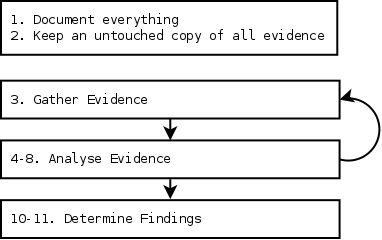
\includegraphics[scale=.75]{./img/Forensics}
\caption{Forensics}
\end{figure}
\begin{enumerate}
\item Document everything.
\item Keep an untouched copy of all evidence.
\item Gather all relevant information
\begin{itemize}
\item Disk images (including memory images) from compromised computers
\item Logs (Windows Event Logs, syslog, web server logs, web client logs, SQL server logs, Remote Desktop logs, SSH logs, etc.) from the compromised computer and other computers
\item Logs from network devices (Firewalls, Intrusion Detection Systems, Anti-malware consoles, etc.)
\item Netflow data from network devices
\end{itemize}
\item Create a calendar and add all relevant dates and times.
\item Run forensics software and a couple anti-malware programs against all disk images. 
\begin{itemize}
\item Redline \url{https://www.mandiant.com/resources/download/redline}
\item Encase \url{https://www.guidancesoftware.com}
\item \url{https://en.wikipedia.org/wiki/EnCase}
\item Please see Malware for more information on anti-malware programs.
\end{itemize}
\item Perform Malware Analysis on any malware. This is a full time job at security or large companies. Alternatively, calculate a hash of all files, and compare these hashes with malware lists.
\begin{itemize}
\item Practical Malware Analysis \url{http://www.nostarch.com/malware}
\item ThreatGRID Malware Analysis and Threat Intelligence \url{http://www.threatgrid.com}
\item National Software Reference Library \url{http://www.nsrl.nist.gov}
\end{itemize}
\item Manually and/or automatically search through the above relevant information for anything interesting. Ask your users for additional information. 
\begin{itemize}
\item Dates
\item IP addresses and URLs
\item Usernames
\item Programs and services
\item Emails
\item Files (Microsoft Office, PDFs, CSVs, etc.)
\end{itemize}
\item Check IP addresses and URLs against malware lists, location information, hostname lists, etc.
\begin{itemize}
\item IP Address Blacklist Checker Tool \url{http://www.ipvoid.com} 
\item ThreatSTOP | Check an IP address \url{http://threatstop.com/checkip}
\item MalwareURL - Website status verification \url{http://www.malwareurl.com/listing-urls.php}
\item Malware Domain List \url{http://www.malwaredomainlist.com/mdl.php}
\item IP Tracker: Lookup, Find, Track \& Trace IP Address \url{http://www.ip-tracker.org}
\item WebHosting.Info's Power WHOIS Service \url{http://whois.webhosting.info}
\end{itemize}
\item Repeat steps 3-8 as necessary.
\item Determine how the computer was compromised.
\item Determine the extent of the compromise.
\begin{itemize}
\item Were other computers compromised from this computer?
\item Was any information exfiltrated from or through this computer?
\end{itemize}
\end{enumerate}
\textbf{Resources}
\begin{enumerate}
\resource[]{Network Security Through Data Analysis}{http://shop.oreilly.com/product/0636920028444.do}
\resource[]{Forensics Wiki}{http://www.forensicswiki.org/wiki/Main_Page}
\resource[]{DD - Wikipedia}{https://en.wikipedia.org/wiki/Dd_(Unix)}
\resource[]{Autopsy}{http://www.sleuthkit.org/autopsy/}
\resource[]{Hex Editor - Wikipedia}{https://en.wikipedia.org/wiki/Hex_editor}
\resource[]{Encase}{https://www.guidancesoftware.com/products/Pages/encase-forensic/overview.aspx}
\resource[]{ProDiscover Basic}{http://www.prodiscover-basic.software.informer.com}
\end{enumerate}
\subsubsection{Malware Reverse Engineering}
\textbf{Resources}
\begin{enumerate}
\resource[]{Cuckoo Sandbox}{http://cuckoosandbox.org}
\resource[]{IDA Pro}{https://www.hex-rays.com/products/ida/index.shtml}
\end{enumerate}
\newpage
\section{Assessments, Audits, and Analyses}\label{sec:"Assessments, Audits, and Analyses"}
Assessments\resourcecite{SecAssTypes} give you the opportunity to take a step back and analyze something: your organization, a process, a computer, a vendor, etc. They also give you insight into the effectiveness of your organization's Information Security Program by identifying the strong and weak areas of your program. Many people use the terms assessment, audit, and analysis interchangeably or give them their own meaning. Generally, assessment refers to risk assessments, network security assessments, and vulnerability assessments. Audit refers to financial audits or a review of logs. And Analysis refers to a HIPAA Security Risk Analysis for Meaningful Use. Also, some people avoid the term audit because employees fear they will fail an audit. Also, employees misinterpret an audit which is a regular check with and investigation which is targeted at a specific wrongdoing.  When you change the term to assessment, everyone calms down a bit.\\\\
In \hyperref[sec:"Your First Day"]{Your First Day} and \hyperref[sec:"Policies and Processes"]{Policies and Processes} we discussed Inventories and Data Flow Diagrams. Use these documents to help frame and start your assessments. You can also use a system model to help define the scope of your assessment. For example, when considering the model below, is your assessment of just the application or do you also want to look at the underlying components:\\
\begin{table}[h]\begin{center}System Model\\\begin{tabular}{|l|}\hline\hline
Application\\\hline
Database\\\hline
Operating System\\\hline
Network\\\hline
Physical\\\hline
\end{tabular}\end{center}\end{table}
\subsection{Risk Assessments}
Risk Assessments are a part of the Risk Management process discussed in Your First Day. First, as with any assessment,  define a scope (network, computer, application). Second, brainstorm all the possible risks to confidentiality, integrity, and availability within that scope. Remember, risk is...
\begin{align}
Risk &= The\ Probability\ a\ Threat\ Source\ Exploits\ a\ Vulnerability \nonumber \\ &\ * The\ Impact\ of\ the\ Vulnerability\ Being\ Exploited
\end{align}
\begin{figure}[h]
\centering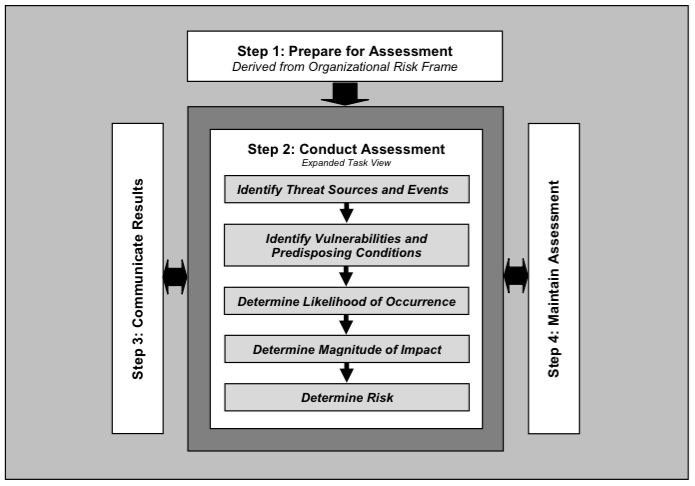
\includegraphics[scale=.55]{./img/RiskAssessmentProcess}
\caption{Risk Assessment Process (NIST Special Publication 800-30 Revision 1)}
\end{figure}
.\\
Define Threat Sources and Threat Events and determine Likelihoods and Impacts of Threat Events. Use the table below to rank and categorize risk.
\begin{figure}[h]
\centering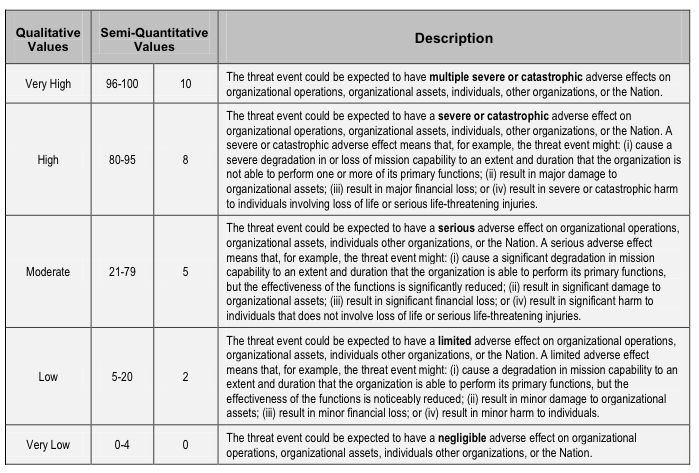
\includegraphics[scale=.55]{./img/QualitativeValues}
\caption{(Risk Values)}
\end{figure}
The formal Risk Assessment process is defined in NIST Special Publication 800-30 Revision 1. Read this document.\\\\
After completing a Risk Assessment, act on the results within the Risk Management Framework. You can respond to  risk and implment controls to midigate the risk or accept the risk and continue to monitor it.
\begin{figure}[h]
\centering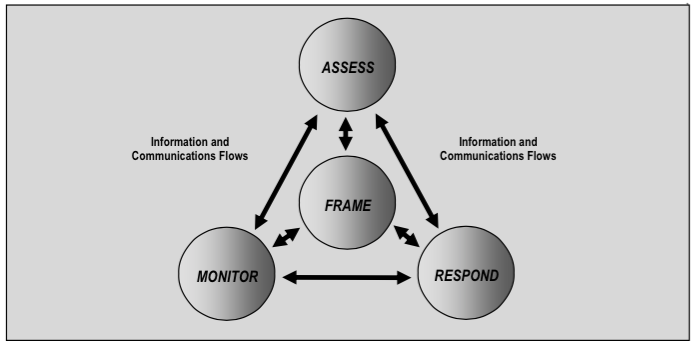
\includegraphics[scale=.55]{./img/RiskManagementProcess}
\caption{Risk Management Process (NIST Special Publication 800-39 \& NIST Special Publication 800-30 Revision 1)}
\end{figure}
\newpage
.
\newpage
.
\newpage
.
\subsubsection{Example Risk Assessment}
\begin{table}[h]\begin{center}\begin{tabular}{|p{1.9cm}|p{2.8cm}|p{1.3cm}|p{1.7cm}|p{1.3cm}|p{2.8cm}|p{1.4cm}|}\hline
Category & Risk & Impact & Likelihood & Risk Value & Mitigating Controls & Residual Risk\\\hline
Policy and Process & Visitor Policy allows visitors to walk around without escorts & Medium & Medium & Medium & Staff trained to keep sensitive information out-of-sight & Low\\\hline
Assessment & No Network Security Assessment allows gaps to go unnoticed & Medium & Medium & Medium & None & Medium\\\hline
Computer & Servers get infected with malware & High & Low & Medium & Anti-virus software & Low\\\hline
... & ... & ... & ... & ... & ... & ... \\\hline
\end{tabular}\end{center}\end{table}
\begin{equation}Risk\ Value = Impact * Likelihood\end{equation}
\begin{equation}Residual Risk = Risk Value - Mitigating\ Controls\end{equation}
\subsection{Gap Analyses}
A Gap Analysis is an assessment performed against an Information Security Standard to determines if the organization is in compliance with the standard. A Gap Analysis is common for any of the Laws, Regulations, and Standards mentioned in Policies and Processes. The product of the assessment lists the areas where the organization's Information Security Program meets the Law, Regulation, or Standard and areas where the organization needs to improve its Program.
\subsection{HIPAA Security Risk Analysis for Meaningful Use}
The HIPAA Security Rule requires all covered entities to annually "conduct an accurate and thorough assessment of the potential risks and vulnerabilities to the confidentiality, integrity, and availability of electronic protected health information held by the [organization]." This assessment is called a HIPAA Security Risk Analysis for Meaningful Use\resourcecite{SRA}\textsuperscript{,}\resourcecite{SRAGuidance}\textsuperscript{,}\resourcecite{SRAT}. It is really a Gap Analysis performed against the HIPAA Security Rule. NIST created a optional toolkit\resourcecite{HIPAATK} to assist in this assessment.
\subsection{Security Testing and Assessments (Offensive Security)}
Security Testing and Assessments incorporates all the activities you take to check every part of your Information Security Program. This is often called Offensive Security because the tester is 'attacking' your information. The rest of the topics in this book are defensive; you are protecting your information.\\\\
There is probably no other area of security that is more discussed or written about than Offensive Security. This section will be short because many other texts cover this section in tremendous depth. Overall, if it exists, you can test it, and you can probably break it.\\\\
Testing\resourcecite{NSA}\textsuperscript{,}\resourcecite{800115} usually follows a three step methodology of reconnaissance, enumeration, and exploitation. First, you locate what you are attacking, next you identify it, and last you break in. This could be accomplished by using nmap\resourcecite{nmap} to scan a netblock, using openvas\resourcecite{openvas} to identity a vulnerability, and using metasploit\resourcecite{metasploit} to exploit that vulnerability. All these tools are open source, but there are thousands of open source and commercial tools for Testing and Assessing.\\\\
Remember to use the System Model described in the beginning of this section to scope your testing and assessments. You may want to limit each engagement to only one network, computer, or application.\\\\
Use the output from your security testing and assessment program to create action. Create tickets for issues that need fixing. Create reports that trend how these programs are performing over time.
\subsubsection{Vulnerability Assessment and Management}
Vulnerability assessments attempt to locate all the vulnerable software on computers on your network. These tools typically have a list of vulnerabilities and attempt to look for each vulnerability on each computer. Your program should include vulnerability management to check the competency of the other parts of your program. However, do not base your patching process on vulnerability management. Vulnerability assessments\resourcecite{vulnpen} are limited to reconnaissance and enumeration.
\subsubsection{Penetration Testing}
Penetration Testing is a goals-driven assessment that attempts to compromise the Confidentiality, Integrity, or Availability of a system. These assessments go beyond reconnaissance and enumeration and exploit any discovered vulnerabilities. Penetration Testing is an essential component of your Risk Management Program. Internal penetration testing teams are called Red Teams while "defensive teams" are Blue Teams. Kali Linux\resourcecite{kali} is a distribution of Linux built for Penetration Testing.
\subsubsection{(Web/Mobile) Application Testing}
An application test, most common against web or mobile applications, is a penetration test limited to one single application. These tests are necessary to evaluate the security controls specific to that application. There are many tools\resourcecite{zap}\textsuperscript{,}\resourcecite{Nikto2}\textsuperscript{,}\resourcecite{Wnikto}\textsuperscript{,}\resourcecite{sqlmap}\textsuperscript{,}\resourcecite{skipfish}\textsuperscript{,}\resourcecite{burp}\textsuperscript{,}\resourcecite{firefoxaddons} and methodologies for these tests.\\
\subsubsection{Social Engineering}
Social Engineering is a test of your employees. These tests often try to trick employees over the phone/text, via email/message, or in person into compromising the Confidentiality, Integrity, or Availability of your information. While many executives do not believe in Social Engineering, these attacks are prevalent in the real world and responsible for many breaches. There are many tools\resourcecite{social}\textsuperscript{,}\resourcecite{phishing}\textsuperscript{,}\resourcecite{set} and methodologies for these tests.\\\\
Phishing is a social engineering attack against an entire company over. It is named because the attacker will cast their hook and lure and hope an employee bites. Spearphishing is a targeted phishing attack: the attacker researches a specific employee before launching the attack. Open Source Intelligence\resourcecite{WOSINT} (OSINT) refers to using information openly available on the Internet for Social Engineering attacks. There are many tools\resourcecite{Metagoofil}\textsuperscript{,}\resourcecite{SpiderFoot}\textsuperscript{,}\resourcecite{FOCA} available.
\subsubsection{Bug Bounty}
Bug Bounties are an external service or external or internal program that rewards researchers for finding bugs. These could be security bugs or other types of bugs. Reward internal employees for reporting bugs by giving them gift cards, t-shirts, etc. Reward your users for reporting bugs by paying them or giving them gift certificates. External services can also coordinate your bug bounty program with public or private researcher groups.\\\\
\textbf{Resources}
\begin{enumerate}
\resource[SecAssTypes]{Security Assessments Types}{https://danielmiessler.com/study/security-assessment-types/}
\resource[SRA]{Security Risk Assessment}{http://www.healthit.gov/security-risk-assessment}
\resource[SRAGuidance]{Guidance on Risk Analysis Requirements under the HIPAA Security Rule}{http://www.hhs.gov/ocr/privacy/hipaa/administrative/securityrule/rafinalguidancepdf.pdf}
\resource[HIPAATK]{HIPAA Security Rule Toolkit}{http://scap.nist.gov/hipaa/}
\resource[SRAT]{Security Risk Analysis Tipsheet}{http://www.cms.gov/Regulations-and-Guidance/Legislation/EHRIncentivePrograms/Downloads/SecurityRiskAssessment_FactSheet_Updated20131122.pdf}
\resource[NSA]{Network Security Assessment: Know Your Network (2nd Edition) By Chris McNab (2007)}{http://shop.oreilly.com/product/9780596006112.do}
\resource[800115]{Special Publication 800-115 Technical Guide to Information Security Testing and Assessment}{http://csrc.nist.gov/publications/nistpubs/800-115/SP800-115.pdf}
\resource[nmap]{nmap}{https://nmap.org}
\resource[openvas]{OpenVAS}{http://www.openvas.org}
\resource[metasploit]{Metasploit}{https://www.metasploit.com}
\resource[vulnpen]{The Difference Between a Vulnerability Assessment and a Penetration Test}{https://danielmiessler.com/essays/vulnerability_assessment_penetration_test/}
\resource[kali]{Kali Linux}{http://www.kali.org}
\resource[zap]{OWASP Zed Attack Proxy Project}{https://www.owasp.org/index.php/OWASP_Zed_Attack_Proxy_Project}
\resource[Nikto2]{Nikto2}{https://cirt.net/Nikto2}
\resource[Wnikto]{Nikto Web Scanner - Wikipedia}{https://en.wikipedia.org/wiki/Nikto_Web_Scanner}
\resource[sqlmap]{sqlmap}{http://sqlmap.org}
\resource[skipfish]{skipfish}{https://code.google.com/p/skipfish}
\resource[burp]{Burp Proxy}{http://portswigger.net/burp/proxy.html}
\resource[firefoxaddons]{Redspin Security Web Assesment Add-ons}{https://addons.mozilla.org/en-US/firefox/collections/nathan-drier/redspin-web/}
\resource[social]{An innovative and comprehensive framework for Social Vulnerability Assessment}{http://www.sicherheitsforschung-magdeburg.de/uploads/journal/MJS_033_Frumento_Assessment.pdf}
\resource[phishing]{Phishing Frenzy}{http://www.phishingfrenzy.com}
\resource[set]{Social Engineer Toolkit (SET)
}{http://www.social-engineer.org/framework/se-tools/computer-based/social-engineer-toolkit-set/}
\resource[WOSINT]{Open Source Intelligence - Wikipedia}{https://en.wikipedia.org/wiki/Open-source_intelligence}
\resource[Metagoofil]{Metagoofil}{http://www.edge-security.com/metagoofil.php}
\resource[SpiderFoot]{SpiderFoot}{http://www.spiderfoot.net/info/}
\resource[FOCA]{FOCA (Fingerprinting Organizations with Collected Archives)}{https://www.elevenpaths.com/labstools/foca/index.html}
\resource{Government Auditing Standards: 2011 Revision}{http://www.gao.gov/assets/590/587281.pdf}
\end{enumerate}
\newpage
\section{Networks}\label{sec:"Networks"}
Salespeople would like for you believe this section is all about gear. It's not. The right gear is often free or inexpensive. More money spent on gear does not equate to a more secure network.
\label{subsec:"Security Zones"}\subsection{Security Zones}
\hyperref[sec:"Your First Day"]{Your First Day} introduced two information security concepts we will now apply to Network Security, the CIA Triad and Information Classification. Networks make information available to many users. We must properly configure controls to protect the confidentiality and integrity of that information. Also, redundancy of network components (multiple internet connections, load balancers, etc.) increases availability.\\\\
The security community often describes information security as an onion. You have to carefully peel back several layers of controls for access to sensitive information. Another phrase for the same concept is defense in depth. The onion analogy works well in network security. In network security, the layers of the onion are security zones defined by Access Control Lists (ACLs) on firewalls. (Some organizations save money by using routers instead of firewalls. Avoid this practice.) ACLs are rules that explicitly allow traffic from one host or network to another host or network (optionally on specific ports). Ideally, we would create a unique security zone for each host and carefully craft ACLs to restrict network traffic to and from that host. However, this would be overly burdensome so we create security zones for similar hosts and group them together. Security zones are visualized with network diagrams. \\\\
Public IP addresses are those that can be routed across the public Internet. These IP addresses are unique to each organization and may not be reused. Private IP addresses\resourcecite{WPN} (also called RFC 1918\resourcecite{RFC1918} addresses) may only be used for internal networks. Network address translation\resourcecite{WNAT} (NAT) allows computers with private address to connect to the public Internet by using the IP address of a gateway. Private IP addresses provides an important security mechanism by allowing internal computers to "hide" behind the gateway. This creates our most basic security zones, public and private. \\\\
Whitelists\resourcecite{WWL} and blacklists\resourcecite{WBL} are two specific Access Control Lists. Whitelists allow all traffic to or from a particular host or network. They can be useful when troubleshooting or performing security testing. However, whitelists are often accidentally left in place longer than necessary. Blacklists, the opposite of whitelists, block all traffic. They are great for protecting networks' confidentiality and integrity, but they severely limit availability. Exceptions are required for every access allowed through the blacklist. In Cisco ACL syntax, whitelists and blacklists are "permit ip any any" and "deny ip any any" respectively.\\\\
Here are the four basic security zones:
\subsubsection{Public / External / Untrusted / Internet}
\begin{description}
\item This security zone is for information suitable for public consumption by everyone in the world. E.g. Internet router, public wifi access
\item Confidentiality risk is not important.
\item Public IP addresses are used for Internet networks.
\end{description}
\subsubsection{DMZ}
\begin{description}
\item This security zone\resourcecite{WDMZ} is for information that has confidentiality risk, but needs to be accessible to authorized users around the world. E.g. Email gateways, web servers
\item Availability and Confidentiality are both important.
\item Public or private IP addressees can be used for DMZ networks.
\item A multi-tier DMZ takes this concept a step further and creates an additional security zone for database servers separate from internet-accessible web servers.
\end{description}
\subsubsection{Private / Internal / Trusted}
\begin{description}
\item This security zone is for information that has confidentiality risk, but does not need to be accessible outside your network. E.g. internal web servers, file servers, database servers, workstations, sensitive information (Protected Health Information, Cardholder Data, etc.)
\item Confidentiality is more important than Availability.
\item Private IP addresses are typically used for internal networks.
\item PCI requires stageful firewalls to protect the cardholder data environment.
\end{description}
\subsubsection{Isolated}
\begin{description}
\item This security zone is for information where confidentiality and integrity risk greatly outweighs availability. E.g. alarm systems, medical devices
\item Isolated networks may have a connection to another network, but access must be strictly controlled. For example, an alarm system may be allowed access out to one host on the Internet. A medical device may not need network access at all.
\item Private IP addresses are typically used for isolated networks.
\end{description} 
\textbf{Assessment}
\begin{description}
\aitem{Test access between security zones to verify Access Control Lists.}
\end{description}
\textbf{Documentation}
\begin{description}
\ditem{Network inventory: document the security zones available on each network device.}
\aitem{Computer inventory: document what security zone each computer belongs in.}
\end{description}
\textbf{Risk Management}\\\\
\begin{tabularx}{\textwidth}{ X | X }
Threats & Controls \\
\hline
\tcitem{Any network attack}{Firewalls with Access Control Lists}
\end{tabularx}\vspace{5mm}
\tccite{Any network attack}{Firewalls with Access Control Lists}
\textbf{Stories}
\begin{description}
\item I connect to a hospital's improperly configured guest wireless network that allows traffic to their private network. An internal file server was also improperly configured to not require authentication and contained files with Protected Health Information (PHI). Anyone within wifi range of the hospital could access PHI without any authentication or logging.
\end{description}
\textbf{Resources}
\begin{enumerate}
\resource[WPN]{Private Network - Wikipedia}{https://en.wikipedia.org/wiki/Private_network}
\resource[RFC1918]{RFC 1918}{http://tools.ietf.org/html/rfc1918}
\resource[WNAT]{Network Address Translation - Wikipedia}{https://en.wikipedia.org/wiki/Network_address_translation}
\resource[WDMZ]{DMZ (Computing) - Wikipedia}{https://en.wikipedia.org/wiki/DMZ_(computing)}
\resource[WWL]{Whitelist - Wikipedia}{https://en.wikipedia.org/wiki/Whitelist}
\resource[WBL]{Blacklist (Computing) - Wikipedia}{https://en.wikipedia.org/wiki/Blacklist_(computing)}
\end{enumerate}
\label{subsec:"Security Zone Examples"}\subsection{Security Zone Examples}
Two basic examples of security zones:
\begin{center}
\begin{figure}[ht]
\begin{verbatim}
                     +------------------+
                     |     Internet     |
                     +------------------+
                              |
                     +------------------+    +-----+
                     |     Firewall     | == | DMZ |
                     +------------------+    +-----+
                              |
                              |             ++----------++
                     +------------------+   ++----------++
                     |     Private      |   || Isolated ||
                     +------------------+   ++----------++
                                            ++----------++
\end{verbatim}
\caption{Use one firewall with three interfaces to create three security zones. The Internet-facing security zone is the least protected, followed by the DMZ, and the Private security zone is the most protected. The isolated zone is not connected to any other security zone.}
\end{figure}
\end{center}
\clearpage
\begin{center}
\begin{figure}[ht]
\begin{verbatim}
                     +------------------+
                     |     Internet     |
                     +------------------+
                              |
                     +------------------+
                     |     Firewall     |
                     +------------------+
                              |
                     +------------------+
                     |       DMZ        |
                     +------------------+ 
                              |
                     +------------------+
                     |     Firewall     |
                     +------------------+
                              |              ++----------++
                     +------------------+    ++----------++
                     |     Private      |    || Isolated ||
                     +------------------+    ++----------++
                                             ++----------++ 
\end{verbatim}
\caption{Use two firewalls with two interfaces each to create three security zones. The Internet-facing security zone is the least protected, followed by the DMZ, and the Private security zone is the most protected. The isolated zone is not connected to any other security zone.}
\end{figure}
\end{center}
\label{subsec:"Internet-accessible Services"}\subsection{Internet-accessible Services}
Internet-accessible services are any services that can be accessed from the public Internet. These services are most likely to be attacked because billions of people on the Internet can access them. Therefore they need extra controls.\\\\
Create a Public IP address request process to document these services in your network inventory. Document the business need, business owner, technical owner, public IP address, private IP address, and ports/services available to the Internet. Verify this information yearly. Services must also be vulnerability scanned before they are opened to the Internet, and they must be rescanned periodically and whenever changes are made.\\\\
Intenet-accessible services belong in a DMZ security zone. They should never be placed in a public security zone or a private security zone because these configuration negate the premise of security zones. Create individual DMZs for each server if possible.\\\\
Only services that need to be accessible to everyone should be allowed access from the Internet. These services include public web servers, public DNS servers, email gateways, VPN endpoints, and video conference gateways. Other services such as internal web servers, file servers, and database servers, must be located in the private security zone and should be remotely accessed by a VPN. Even this access should only be allowed if necessary. (Please see the section \hyperref[subsec:"Virtual Private Networks"]{Virtual Private Networks} below for more information on VPNs.) Services such as  web mail are often Internet-accessible. However, this configuration allows anyone access to break into web mail which usually contains sensitive information. Instead put these services in a private security zone and require a VPN to access them.\\\\
Run two sets of DNS services to separate public DNS from private DNS. This configuration is referred to as split-DNS. Public DNS servers must not provide private IP addresses for computers in your DMZ or private security zones.\\\\
\textbf{Assessment}
\begin{description}
\aitem{Ping scan your public IP address space from outside your network to see what hosts respond.}
\begin{verbatim}nmap -–sP 1.2.3.0/24\end{verbatim}
\aitem{Port scan your public IP address space from outside your network to see what services respond.}
\begin{verbatim}nmap 1.2.3.0/24\end{verbatim}
\end{description}
\textbf{Documentation}
\begin{description}
\ditem{Network Inventory: Document the business need, business owner, technical owner, public IP address, private IP address, and ports/services for each internet-accessible service.}
\end{description}
\textbf{Risk Management}\\\\
\begin{tabularx}{\textwidth}{ X | X }
Threats & Controls \\
\hline
Any internet attack & Public IP address request process \\ & Vulnerability scans\\ & Firewalls with Access Control Lists
\end{tabularx}\vspace{5mm}
\textbf{Stories}
\begin{description}
\item Many organizations allow access to webmail services to anyone on the internet. A simple social engineering attack provides access to a user's email account.
\item An organization improperly allowed internet access to their development web server that was running out-of-date software and was configured with default credentials. This server could then access the properly secured production web servers that contained sensitive information.
\end{description}
\subsection{Internal Access Control}
Creating a strong perimeter is only part of building a secure network. Onions have multiple layers. Internal Access Control limits access between computer in the private security zone. Often, the greatest threats are within your own organization: your employees' compromised computers for example.\\
Within the private security zone, create additional security zones to protect high-risk computers. Use Access Control Lists on internal firewalls or routers to control access between separate Virtual LANs\resourcecite{WVLAN} (VLANs) for separate computers. Very high-risk computers should be placed in isolated security zones.\\\\
Some organizations have a process for requesting private IP addresses and access to the private security zone similar to the process described above for public IP addresses. This is recommended, but not required.
\subsubsection{Host-based Firewalls}
A host-based firewall is a software firewall running on a computer that allows you to create Access Control Lists for that specific computer. Depending on the host-based firewall, you can create ingress rules, egress rules, or both. They are the closest most organizations can get to creating a security zone for each computer. Common host-based firewalls include Windows Firewall, Mac OS X's firewall, and Linux's IP Tables\resourcecite{WIPTables}. Host-based firewalls should be enabled on all computers on your network.
\subsubsection{Network Access Control}\label{subsubsec:"Network Access Control"}
Network Access Control\resourcecite{WNAC} (NAC) prevents unauthorized users with physical access to a ethernet port from accessing your network. Newer systems can also require computers to be running up-to-date anti-virus or other software before they are allowed network access. They can even assign a computer to a specific VLAN based on these checks. The underlying protocol behind network access control is IEEE 802.1X\resourcecite{W8021x} and it typically requires a RADIUS server for user management. Users have to enter their username and password, or other credentials, to access the network. Network access control is rarely implemented. If you don't use NAC, disable all unused Ethernet ports. It is also possible to control network access by limiting the MAC addresses of computers that are allowed access to the network, limiting MAC addresses of computers that are given DHCP addresses, and/or requiring static IP addresses. However, all of these techniques can be easily circumvented by copying a MAC address or IP address from an existing computer.\\\\
\textbf{Assessment}
\begin{description}
\aitem{Ensure high-risk computers have additional network protections.}
\aitem{Ensure all computer are running host-based firewalls.}
\aitem{Attempt to gain access to the network from publicly-accessible Ethernet ports in a lobby, conference room, or cafeteria.}
\end{description}
\textbf{Documentation}
\begin{description}
\ditem{Computer inventory: Document any additional network protections for high-risk computers.}
\end{description}
\textbf{Risk Management}\\\\
\begin{tabularx}{\textwidth}{ X | X }
Threats & Controls \\
\hline
\tcitem{Attacks from within the private security zone}{Internal Access Control and Host-based firewalls}
\tcitem{Publicly-accessible Ethernet ports}{Network Access Control}
\end{tabularx}\vspace{5mm}
\textbf{Stories}
\begin{description}
\item I walk into a bank's conference room and plug a laptop into their Ethernet port. When asked by a branch manager why I am there, I reply "I'm here early for a meeting." Her response is "OK, just don't plug your computer into the wall" although she doesn't see it is already connected. Thankfully they have Network Access Control which prevents my computer from accessing their network.
\end{description}
\textbf{Resources}
\begin{enumerate}
\resource[WVLAN]{VLAN - Wikipedia}{https://en.wikipedia.org/wiki/Vlan}
\resource[WIPTables]{IP Tables - Wikipedia}{https://en.wikipedia.org/wiki/Iptables}
\resource[WNAC]{Network Access Control - Wikipedia}{https://en.wikipedia.org/wiki/Network_access_control}
\resource[W8021x]{802.1x - Wikipedia}{https://en.wikipedia.org/wiki/802.1x}
\end{enumerate}
\subsection{Wireless}\label{subsec:"Wireless"}
Most organizations provide wireless network\resourcecite{WWLAN}\textsuperscript{,}\resourcecite{W80211} access to their employees and/or guests. Wireless is a convenient way to access the network. Wireless can be configured in the following three ways (with accompanying security zone): employee wireless (internal), guest wireless (public), and isolated wireless (isolated). These networks should be created on separate SSIDs.
\subsubsection{Employee wireless}
Configure this network so clients can access the private security zone. Use Wi-Fi Protected Access 2\resourcecite{WWPA} (WPA2) to authenticate access to the network and encrypt communications. There are two versions of WPA2: WPA2 Personal and WPA2 Enterprise. As their names imply, WPA2 Personal is designed for home or small office use. WAP2 Enterprise is designed for large organization with centralized authentication services.\\
\begin{mdframed}\begin{tabularx}{\textwidth}{ p{1.9cm} | p{2.8cm} | p{2.3cm} | p{2.2cm} | p{2cm} }
 & Authentication & Pros & Cons & Encryption \\
\hline
WPA2 Personal & Pre-shared key &  Easy setup & Shared password & AES \\
\hline
WPA2 Enterprise & 802.1X & Individual accounts & Requires RADIUS server & AES
\end{tabularx}\end{mdframed}
Do not use Wired Equivalent Privacy\resourcecite{WWEP} (WEP) or WPA. They rely on less secure authentication and encryption protocols. Additionally, hidden SSIDs\resourcecite{WSSID} are not an effective control: they are easy to find.\\\\
Train employees to use the employee wireless network and not the guest wireless network.
\subsubsection{Guest wireless}
Configure guest wireless so clients can only access the public security zone.
\subsubsection{Isolated wireless}
Isolated wireless networks must only be created for a specific need. Configure isolated wireless so clients cannot access public or private security zones.
\subsubsection{Rouge access points}
Rogue access points\resourcecite{WRogue} are unauthorized wireless networks. There are two types:
\begin{itemize}
\item Access points connected to the private security zone that allow unauthorized access to the private security zone.
\item Access points named similar to authorized access points that attempt to trick your employees to join them. These networks are used for man-in-the-middle attacks.
\end{itemize}
Periodically assess your locations for rogue access points. There are products to help automate these assessments.\\\\
\textbf{Assessment}
\begin{description}
\aitem{Ensure employee, guest, and isolated wireless networks are in the correct security zones and do not have access to unauthorized security zones.}
\aitem{Ensure the employee wireless network requires authentication and encrypts traffic.}
\aitem{Ensure employees are not using the guest wireless network.}
\aitem{Ensure there are no rouge access points within wireless range.}
\end{description}
\textbf{Documentation}
\begin{description}
\ditem{Information security policy: Do not allow rogue access points.}
\end{description}
\textbf{Risk Assessment}\\\\
\begin{tabularx}{\textwidth}{ l | X }
Threats & Controls \\
\hline
\tcitem{Weak Encryption}{WPA2}
\tcitem{Any attack from guest wireless}{Firewalls with Access Control Lists}
\tcitem{Rouge access points}{Periodic scans for rouge access points} 
\end{tabularx}\vspace{5mm}
\tccite{Weak Encryption}{WPA2}
\tccite{Any attack from guest wireless}{Firewalls with Access Control Lists}
\tccite{Rouge access points}{Periodic scans for rouge access points} 

\textbf{Resources}
\begin{enumerate}
\resource[WWLAN]{Wireless LAN - Wikipedia}{https://en.wikipedia.org/wiki/Wireless_LAN}
\resource[W80211]{IEEE 802.11 - Wikipedia}{https://en.wikipedia.org/wiki/IEEE_802.11}
\resource[WWPA]{Wi-Fi Protected Access - Wikipedia}{https://en.wikipedia.org/wiki/Wi-Fi_Protected_Access}
\resource[WWEP]{Wired Equivalent Privacy - Wikipedia}{https://en.wikipedia.org/wiki/Wired_Equivalent_Privacy}
\resource[WSSID]{Service set (802.11 network) - Wikipedia}{https://en.wikipedia.org/wiki/Service_set_(802.11_network)}
\resource[WRogue]{Rogue Access Point - Wikipedia}{https://en.wikipedia.org/wiki/Rogue_access_point}
\end{enumerate}
\subsection{Virtual Private Networks}\label{subsec:"Virtual Private Networks"}
A Virtual Private Network\resourcecite{WVPN} (VPN) is a way to bridge two private security zones across a public security zone. This is typically done by encrypting all traffic that traverses the public security zone. VPNs are used to connect a company's network between remote sites, to connect two different companies' networks, or to allow users to remotely connect to their company's network.
\begin{verbatim}
                     +------------------+
                     |     Private      |
                     +------------------+
                              |
                     +------------------+
                     |    VPN Device    |
                     +------------------+
                             | |
                         (encrypted)
                             | |
                     +------------------+
                     |      Public      |
                     +------------------+ 
                             | |
                         (encrypted)
                             | |
                     +------------------+
                     |    VPN Device    |
                     +------------------+
                              |             
                     +------------------+ 
                     |     Private      | 
                     +------------------+ 
\end{verbatim}
VPNs used to be created using the Point-to-Point Tunneling Protocol\resourcecite{WPPTP} (PPTP) and then the Layer 2 Tunneling Protocol\resourcecite{WL2TP} (L2TP). These protocols are built into Windows, Mac OS, and Linux. However, they do not explicitly require encryption and have other shortcomings. Most modern VPNs use IP Security\resourcecite{WIPSec} (IPSec). They should also use AES for the encryption protocol if possible.\\\\
A VPN that connects different sites within one company should implement the same internal access control as described above. However, also consider that differences in physical security, network access control, or other issues between different sites may require different internal access controls.\\\\
A VPN that connects two different companies across the Internet must also implement access control. Both companies should create the VPN in their respective DMZ networks. Access to internal resources should be explicitly allowed just as with other systems located in a DMZ.
\subsubsection{Remote Access}
Remote access allows users from an untrusted network such as the Internet to access resources behind the perimeter. This is fundamentally against everything discussed in \hyperref[subsec:"Security Zones"]{Security Zones}. This should give you pause. However, remote access is often a necessity.\\\\
Remote access was originally accomplished through something like Telnet\resourcecite{WTelnet}. However, most users want a graphical user interface, Telnet is unencrypted, and Telnet authentication is typically just a username and password. For these reasons, modern remote access is typically configured to use a VPN, either and IPSec VPN or an SSL VPN. As noted above, either option should be configured to use AES.  Also, consider requiring multi-factor authentication for remote access. Please see \hyperref[subsubsec:"Authentication"]{Authentication} for more infomation on multi-factor authentication. PCI requires multi-factor authentication for remote access to the cardholder data environment.\\\\
Also, remote access should not allow complete access to the internal network. Remote access users should be placed in a DMZ network with access to limited services such as email and file servers. Create multiple DMZs for different user roles if necessary. Many organizations allow remote access users to connect to their desktop computers at the office via a protocol such as Microsoft's Remote Desktop\resourcecite{WRDS}, Virtual Network Computing\resourcecite{WVNC} (VNC), or Secure Shell\resourcecite{WSSH} (SSH).  They can then access any internal resources from their desktop. Some organizations  publish a Citrix\resourcecite{WCitrix} desktop to remote access users. This may be the same Citrix desktop they use at work.\\\\
Some organizations only allow remote access from company computers because personal computers may not be running the same security software or configurations. Additionally, some organizations require users to sign a separate acceptable use agreement governing remote access.
\\\\Many users are opting to use personal remote access products such as Go2MyPC for remote access. These products create a backdoor into the internal network. Restrict the use of these products in your acceptable use policy and consider monitoring the network for traffic using these services.\\\\
\textbf{Resources}
\begin{enumerate}
\resource[WVPN]{Virtual Private Network - Wikipedia}{https://en.wikipedia.org/wiki/Virtual_private_network}
\resource[WPPTP]{PPTP - Wikipedia}{https://en.wikipedia.org/wiki/Pptp}
\resource[WL2TP]{L2TP - Wikipedia}{https://en.wikipedia.org/wiki/L2TP}
\resource[WIPSec]{IPSec - Wikipedia}{https://en.wikipedia.org/wiki/Ipsec}
\resource[WTelnet]{Telnet - Wikipedia}{https://en.wikipedia.org/wiki/Telnet}
\resource[WRDS]{Remote Desktop Services - Wikipedia}{https://en.wikipedia.org/wiki/Remote_Desktop_Services}
\resource[WVNC]{VNC - Wikipedia}{https://en.wikipedia.org/wiki/Vnc}
\resource[WSSH]{Secure Shell - Wikipedia}{https://en.wikipedia.org/wiki/Secure_Shell}
\resource[WCitrix]{Citrix XenAPP - Wikipedia}{https://en.wikipedia.org/wiki/Citrix_XenApp}
\end{enumerate}
\subsection{Network Devices}
This is the gear section. Time to break out the checkbook. Unless you're the open source type in which case most of the gear you need is a COTS PC. Follow your \hyperref[subsec:"Network Device Hardening Process"]{Network Device Hardening Process} when configuring network devices.
\subsubsection{Application Firewalls}
Application Firewalls\resourcecite{WAF} are network security devices that monitor and manipulate traffic higher than layer 3/4. Web Application Firewalls are the most common Application Firewalls and they can prevent common web application attacks. Please see \hyperref[subsec:"Internally-developed Applications"]{Internally-developed Applications} for more information on web application attacks.
\subsubsection{Logging and Monitoring}
Configure all your network devices to log\resourcecite{80092} to a central server using Syslog\resourcecite{WSyslog}. Consider several Syslog servers for different security zones. Additionally, configure all network devices for Network Time Protocol (NTP)\resourcecite{WNTP}. NTP guarantees logs from different devices reference the same time source. Also configure server logs to log to a central server. Monitor these logs regularly for any anomalies. Simple Network Management Protocol (SNMP)\resourcecite{WSNMP} provides similar logging functionality to Syslog. Last, Nagios\resourcecite{Nagios}\textsuperscript{,}\resourcecite{WNagios} is a great network monitoring tool.\\\\
Network traffic can be viewed as Netflow\resourcecite{WNetflow}\textsuperscript{,}\resourcecite{NetflowTools} (or IPFIX\resourcecite{WIPFIX} or sFlow\resourcecite{WsFlow}) or packet captures (pcap)\resourcecite{WPcap}. Netflow data is available from many types of network devices and is limited to little more than source and destination information. Pcap files, on-the-other-hand, contain entire packets. Most organizations can store Netflow data from critical firewalls and routers for a year or more. However, pcap data for one or two critical links can often only be stored for a week because of storage limitations. Pcap files from network device links are often created by IDS or IPS devices (see below). Pcap files can also be created on a computer's own network links using tcpdump\resourcecite{Wtcpdump} or Wireshark\resourcecite{WWireshark}\resourcecite{NoWireshark}. Also, ngrep\resourcecite{Wngrep} is a great tool for searching inside pcap files similar to grep for regular files. Use SiLK\resourcecite{SiLK} to investigate Netflow data.
\subsubsection{Intrusion Detection and Intrusion Prevention}
Intrusion detection (IDS)\resourcecite{WIDS}\textsuperscript{,}\resourcecite{80094} refers to a device's capability to detect malicious network traffic through pattern recognition, signatures, or other methods. Often network traffic from core switches and routers will be mirrored to an IDS. Intrusion prevention (IPS)\resourcecite{WIPS} takes IDS a step further by actively reconfiguring access control lists to block malicious traffic. The risk of an IPS is that availability may be compromised if legitimate traffic is blocked. However, confidentiality, availability, or integrity of the network as a whole may be increased. All of these systems must be tuned to work effectively in your environment. IDS and IPS capabilities can be built into network devices such as firewalls or separate stand-alone devices. IDS and IPS logs must be sent to a central logging server just like other network devices and servers. Snort\resourcecite{Snort}\textsuperscript{,}\resourcecite{WSnort} and Suricata\resourcecite{Suricata} an open source IDS.\\\\
There are typically three ways an IDS or IPS device can be connected to your network: inline transparent, inline routing, or tap. The two inline modes work by connecting a network link through the IDS or IPS device. In the transparent mode, the device does not modify traffic except when traffic is blocked. In routing mode, the device functions a router and can also block traffic. In tap mode, the device is connected to a mirrored port on another network device such as a firewall, router, or switch. The other device copies all traffic through one or more ports and sends that copy out the mirrored port. All IDS and IPS devices in tap mode cannot block traffic and function as IDS devices only.\\\\
Security Onion\resourcecite{SecurityOnion} is a Linux distribution that offers intrusion detection, network monitoring, and logging.
\subsubsection{Security Information and Event Management}
Security Information and Event Management (SIEM)\resourcecite{WSIEM} refers to a more comprehensive logging and monitoring solution. These systems typically correlate logs and alerts from numerous types of network devices, servers (Windows Event Logs and Syslogs), and application and attempt to tie together security events.
\subsubsection{Proxy Servers and Web Filters}
Proxy servers intercept communications between users and servers. The most common proxy server is a caching web proxy server. This server intercepts all the web traffic leaving the perimeter. The server can then respond quicker to user requests if it sees two users that are visiting the same site. Some organizations require all web traffic to go through proxy servers so they can filter the traffic. Other organizations buy devices that are purpose-built for filtering web traffic. All of these devices can be used to enforce policies regarding web access. Web Cache Communication Protocol (WCCP)\resourcecite{WWCCP} is a control that can automatically send web traffic through a proxy server.
\subsubsection{Data Loss Prevention}\label{subsubsec:"Data Loss Prevention"}
Data loss prevention (DLP)\resourcecite{WDLP} is a category of software that attempts to locate sensitive data and detect and limit where it can go. DLP usually operates by scanning files servers and computers connected to the network, or by listening to network traffic, or both.\\\\
\textbf{Resources}
\begin{enumerate}
\resource[WAF]{Application Firewall - Wikipedia}{https://en.wikipedia.org/wiki/Application_firewall}
\resource[80092]{NIST Special Publication 800-92 Guide to Computer Security Log Management}{http://csrc.nist.gov/publications/nistpubs/800-92/SP800-92.pdf}
\resource[WSyslog]{Syslog - Wikipedia}{https://en.wikipedia.org/wiki/Syslog}
\resource[WNTP]{Network Time Protocol - Wikipedia}{https://en.wikipedia.org/wiki/Network_Time_Protocol}
\resource[WSNMP]{Simple Network Management Protocol - Wikipedia}{https://en.wikipedia.org/wiki/Snmp}
\resource[Nagios]{Nagios}{http://www.nagios.org}
\resource[WNagios]{Nagios - Wikipedia}{https://en.wikipedia.org/wiki/Nagios}
\resource[WNetflow]{Netflow - Wikipedia}{https://en.wikipedia.org/wiki/Netflow}
\resource[NetflowTools]{Freeware NetFlow Software - Cisco}{http://www.cisco.com/c/en/us/products/ios-nx-os-software/ios-netflow/networking_solutions_products_genericcontent0900aecd805ff72b.html}
\resource[WIPFIX]{IP Flow Information Export}{https://en.wikipedia.org/wiki/IP_Flow_Information_Export}
\resource[WsFlow]{SFlow - Wikipedia}{https://en.wikipedia.org/wiki/SFlow}
\resource[WPcap]{Pcap - Wikipedia}{https://en.wikipedia.org/wiki/Pcap}
\resource[Wtcpdump]{tcpdump - Wikipedia}{https://en.wikipedia.org/wiki/Tcpdump}
\resource[WWireshark]{Wireshark - Wikipedia}{https://en.wikipedia.org/wiki/Wireshark}
\resource[NoWireshark]{No Wireshark? No TCPDump? No Problem!}{https://isc.sans.edu/diary/No+Wireshark\%3F+No+TCPDump\%3F+No+Problem\%21/19409}
\resource[Wngrep]{ngrep - Wikipedia}{https://en.wikipedia.org/wiki/Ngrep}
\resource[SiLK]{SiLK}{http://tools.netsa.cert.org/silk/index.html}
\resource[WIDS]{Intrusion Detection System - Wikipedia}{https://en.wikipedia.org/wiki/Intrusion_detection_system}
\resource[80094]{NIST Special Publication 800-94 Guide to Intrusion Detection and Prevention Systems (IDPS)}{http://csrc.nist.gov/publications/nistpubs/800-94/SP800-94.pdf}
\resource[WIPS]{Intrusion Prevention System - Wikipedia}{https://en.wikipedia.org/wiki/Intrusion_prevention_system}
\resource[Snort]{Snort}{https://www.snort.org}
\resource[WSnort]{Snort - Wikipedia}{https://en.wikipedia.org/wiki/Snort_(software)}
\resource[Suricata]{Suricata}{http://suricata-ids.org}
\resource[SecurityOnion]{Security Onion}{http://blog.securityonion.net/p/securityonion.html}
\resource[WSIEM]{Security Information and Event Management - Wikipedia}{https://en.wikipedia.org/wiki/Security_Information_and_Event_Management}
\resource[WWCCP]{Web Cache Communication Protocol - Wikipedia}{https://en.wikipedia.org/wiki/Web_Cache_Communication_Protocol}
\resource[WDLP]{Data Loss Prevention - Wikipedia}{https://en.wikipedia.org/wiki/Data_loss_prevention_software}
\resource{http://www.fluentd.org}{fluentd}
\resource{Port Mirroring - Wikipedia}{https://en.wikipedia.org/wiki/Port_mirroring}
\end{enumerate}
\newpage
\section{Computers}\label{sec:"Computers"}
Computers: servers, workstations, laptops, tablets, smartphones, etc. The human-interface devices of your information. Organize your computers in the proper network security zones. Don't put computers in multiple security zones. Use each computer for one task only. For example, run a separate web server and an email server. Use one workstation as an administrator and another to check your email.\\\\
Computer security starts with your  \hyperref[subsec:"Computer Hardening Process"]{Computer Hardening Process}. The next step in the \hyperref[subsubsec:"Computer Lifecycle"]{Computer Lifecycle} is to maintain your computers. Last follow your \hyperref[subsec:"Disposal and Retention"]{Disposal Policy} for computers. Ensure all computers and applications are in your inventory and you have strong policies around the management of these.
\subsection{Management}
Managing one computer is easy. Managing more than one is difficult. Utilize a management solution tailored to your needs. Use Active Directory\resourcecite{WAD} and Group Policy Objects (GPOs) for Windows computers. Consider using Open Directory\resourcecite{WOD} or JAMF CasperSuite\resourcecite{JAMF} for Macs. Use Puppet\resourcecite{Puppet} or Chef\resourcecite{Chef} for Linux servers. (Puppet also supports Windows.) Use mobile-device management (MDM) to manage mobile devices. These management solutions automate and document the rest of the sections in this chapter.
\subsubsection{Pets and Cattle}
Due to the proliferation of virtual machines and cloud computing, Microsoft's Bill Baker created the terms Pets and Cattle. Pet administrators manage each computer individually and with great care. When a computer breaks, they fix it. Cattle administrators treat computers as disposable assets. If one gets sick, re-image it. This mentality can help with management. It is often quicker to redeploy a server than remove a virus or install a patch.
\subsection{Malware}
Malicious Software (malware) is any virus, worm, or trojan. Malware could be an standalone application, embedded in an application, or embedded in a document. Run an up-to-date version of your favorite anti-malware\resourcecite{WAV} program on all computers to help prevent and contain malware. Many malware products include management consoles to help distribute signatures and updates. Ensure antivirus software is always up-to-date.\\\\
Malware comes from different sources: the Internet, other computers on the network, malicious flash drives, etc. Educate employees on how to detect suspicious websites and not to connect flash drives or other media from untrusted sources. Also educate employees how to respond to suspected malware.\\\\
EICAR\resourcecite{EICAR} is a malware test file. The 68 character string saved as a text file should be detected by all anti-malware programs.
\begin{center}
\begin{figure}[ht]
\begin{verbatim}
X5O!P%@AP[4\PZX54(P^)7CC)7}$EICAR-STANDARD-ANTIVIRUS-TEST-FILE!$H+H*
\end{verbatim}
\caption{EICAR}
\end{figure}
\end{center}
\subsection{Patching (Externally-developed Applications)}
Applying security patches\resourcecite{80040}\textsuperscript{,}\resourcecite{WPatch} is the most effective method of protecting computers from known security vulnerabilities. However, patching doesn't fix everything: zero-day vulnerabilities are software exploits for which no patch is available.\\\\
Patching all software on all computers is usually a large undertaking. Also, because patches are released often, they must be applied often. Patch management solutions help to drastically reduce the workload of patching. Also, most operating systems have a built-in patching functionality such as Windows Updates\resourcecite{WWU} and Windows Server Update Services\resourcecite{WWSUS} for Microsoft Windows or Apple Software Update\resourcecite{WASU} and the Mac App Store\resourcecite{WMAS} for Mac OS X. Linux computers have apt, yum, or anther tool.\\\\
Patching can cause issues with software compatibility, however, this has lessened in recent years. However, it is still advisable to test patches on a subset of computers before deploying to all computers.\\\\
Client-side attacks are attacks against users' computers instead of servers. Web-based client-side attacks commonly attempt to exploit vulnerabilities in out-of-date web browsers or plug-ins such as Adobe Flash or Oracle Java. Because these attacks are common against all computers on the Internet, patching is important for all computers connected to the Internet. These attacks are also not typically prevented by firewalls or intrusion prevention systems.
\subsection{Internally-developed Applications}\label{subsec:"Internally-developed Applications"}
Patching is important for externally-developed applications, but what about internally-developed applications\resourcecite{WAppSoftware}? Implement security in your Software Development Lifecycle. Use training\resourcecite{alert1} to educate your developers about secure coding practices. Inventory all your applications. Continuously perform (web) application assessments on applications. (The OWASP Top 10\resourcecite{OWASPTop10} is included as an appendix.) Perform code reviews on your source code. Require developers to review eachother's code.
\subsection{Logging and Monitoring}
Configure all log sources (Application Logs, Windows Event Logs, Mac/Linux Syslogs, Network Device Syslog, Netflow, etc.) to log to a central log collector. This protects logs from tampering or destruction and allows you to analyse events from different systems. Next, implement a mechanism to process and analyse logs such as the Elasticsearch, Logstash, and Kibana (ELK)\resourcecite{ELK} platform. Regularly check logs.
\subsection{Backups}
If encrypt, encrypt, encrypt is the mantra of confidentiality, and hash, hash, hash is the mantra of integrity, then backup, backup, backup is the mantra of availability. Perform routine backups and store backups off-site by backing up to a remote site or by moving encrypted back medium to a secure location. Follow DR/BCP documentation and retention policies to determine what to backup, how often to back it up, and when to destroy backups.\\\\
\textbf{Assessment}
\begin{description}
\aitem{Verify up-to-date anti-malware software is installed on all computers on the network. Many vulnerability scanners will automate this task by providing a list of all installed software on all computers.}
\aitem{Vulnerability scan all computers on the network to verify all software is up-to-date.}
\end{description}
\textbf{Documentation}
\begin{description}
\ditem{Document installation of anti-malware software in the System Hardening Process.}
\ditem{Require all guest computers on the network to run up-to-date anti-malware software.}
\ditem{Train employees not to visit suspicious websites or use suspicious flash drives.}
\ditem{Create a policy that requires all software on all computers on the network to be up-to-date.}
\ditem{Document a procedure to patch all computers on the network. Consider an automated patch management solution.}
\end{description}
\textbf{Risk Management}\\\\
\begin{tabularx}{\textwidth}{ l | X }
Threats & Controls \\
\hline
\tcitem{Malware}{Install anti-malware software on all computers}
\tcitem{Publicly known software exploit}{Remove unnecessary software and patch all installed software}
\end{tabularx}\vspace{5mm}
\tccite{Malware}{Install anti-malware software on all computers}
\tccite{Publicly known software exploit}{Remove unnecessary software and patch all installed software}
\textbf{Resources}
\begin{enumerate}
\resource[WAD]{Active Directory - Wikipedia}{https://en.wikipedia.org/wiki/Active_Directory}
\resource[WOD]{Apple Open Directory - Wikipedia}{https://en.wikipedia.org/wiki/Apple_Open_Directory}
\resource[JAMF]{JAMF CasperSuite}{http://www.jamfsoftware.com/products/casper-suite/}
\resource[Chef]{Chef}{https://www.chef.io}
\resource[Puppet]{Puppet Labs}{https://puppetlabs.com}
\resource[WAV]{Anti-virus - Wikipedia}{https://en.wikipedia.org/wiki/Anti-virus}
\resource[EICAR]{EICAR}{http://www.eicar.org/86-0-Intended-use.html}
\resource[80040]{NIST Special Publication 800-40 Revision 3 Guide to Enterprise Patch Management Technologies}{http://nvlpubs.nist.gov/nistpubs/SpecialPublications/NIST.SP.800-40r3.pdf}
\resource[WPatch]{Patch - Wikipedia}{https://en.wikipedia.org/wiki/Patch_(computing)}
\resource[WASU]{Apple Software Update - Wikipedia}{https://en.wikipedia.org/wiki/Apple_Software_Update}
\resource[WMAS]{Mac App Store - Wikipedia}{https://en.wikipedia.org/wiki/Mac_App_Store}
\resource[WWSUS]{Windows Server Update Services - Wikipedia}{https://en.wikipedia.org/wiki/Windows_Server_Update_Services}
\resource[WWU]{Windows Update - Wikipedia}{https://en.wikipedia.org/wiki/Windows_Update}
\resource[WAppSoftware]{Application Software - Wikipedia}{http://en.wikipedia.org/wiki/Application_software}
\resource[OWASPTop10]{OWASP Top 10}{https://www.owasp.org/index.php/Top_10_2013-Top_10}
\resource[alert1]{alert(1) to win}{http://escape.alf.nu}
\resource[ELK]{ELK Stack Download}{https://www.elastic.co/downloads}
\end{enumerate}
\newpage
\section{Identity and Access Management}\label{sec:"Identity and Access Management"}
\subsection{Access Control}
\subsubsection{Role-based access control}\textbf{Role-based access control}\resourcecite{WAC}\textsuperscript{,}\resourcecite{WRBAC} is using groups to assign access. When you create a user, put them in groups that automatically control access. For example the "Doctor" group provides read/write access to the Electronic Medical Record. Users in the "Administrator" group often have unrestricted access.
\subsubsection{Separation/Segregation of duties}\textbf{Separation/Segregation of duties}\resourcecite{WSOD} is a control where no one person can single-handily take action to an damage an organization, intentionally or unintentionally.  For example, when granting a user access to an application, separate people should request, grant, implement, and audit access. The same process should be followed when creating access-control lists. When pushing code to production, a developer should not have direct access to production servers. 
\subsubsection{Identification}\textbf{Identification} is the process by which a person or service makes a claim of identity. A username is a common method of identification. Identification does not provide any verification.
\subsubsection{Authentication}\label{subsubsec:"Authentication"}\textbf{Authentication} is the process of verifying a person or service is who he or she claims to be. There are three factors that can be used to authenticate an account: something you know, something you have, and something you are.\\\\
\textbf{Something you know} is a password, pass phrase, or personal identification number. It is a string of letters, numbers, characters, etc. that only you know. Something you know can be guessed. Problems with this factor include people choosing poor passwords, people forgetting passwords, people writing down passwords, and people giving others their passwords.\\\\
\textbf{Something you have} is a token, certificate, (smart) card, or phone number. It is a physical or digital string that only you have. Something you have can be stolen or duplicated.\\\\
\textbf{Something you are} is a retina scan, fingerprint, voice print, etc. It is a biometric signature that only you have. Something you are is hard to guess or steal, but it is also hard to input: most computers do not come with fingerprint scanners or retina scanners.\\\\
\textbf{Where you are} is gaining traction as a fourth distinct factor for mobile devices.\\\\
\textbf{Two-factor authentication} is any combination of two distinct factors such as a debit card and a PIN or a password and a digital certificate. Two-factor authentication is used when greater security is needed such as for large transactions, prescribing controlled substances, or remote access. Using two of the same factor, such as two passwords, does not provide the same increase in security and should be avoided. The DEA requires FIPS-approved two-factor authentication for Electronic Prescribing of Controlled Substances. PCI requires two-factor authentication for remote access.
\subsubsection{Authorization}\textbf{Authorization} is the process of verifying a person or service has access to a specific resource. A user may have an domain account, but they must also be specifically authorized to access email or a file share. Authorization is typically controlled through an Access Control List (ACL) placed on an account or group of accounts.
\subsubsection{Accounting}\textbf{Accounting}
Accounting is the process of tracking what accounts accessed what resources. This is often done automatically, but is also often disabled by default. Accounting  of access to medical records is usually called auditing and contains more detail about what specific actions a user performed.
\subsection{Single Sign-on}\textbf{Single Sign-on} (SSO) is a category of technologies that allow users to login to their computer once and use their session to login to all other applications. Apple's Keychain is an example.
\subsection{Inactivity Timeouts}\textbf{Inactivity Timeouts} are a mechanism to disable access to information after a specific amount of inactivity time. These could be an operating system screensaver timeout or an automatic logout from an application. 
\subsection{Account Management}
\subsubsection{Directory Services}
Almost all large organizations use a directory service\resourcecite{WDS} to store and manage user accounts. Most modern directory services are based on the Lightweight Directory Access Protocol (LDAP)\resourcecite{WLDAP} including Microsoft's Active Directory. The directory attempts to act as the single-sign-on account mechanism. However, in practice, most organizations rely on multiple directories and/or local accounts for some applications.\\\\
RADIUS\resourcecite{WRADIUS} servers, discussed in \hyperref[subsubsec:"Network Access Control"]{Network Access Control} and \hyperref[subsec:"Wireless"]{Wireless}, can also be tied to your directory service to support 802.1X network authentication for wired or wireless networks. Common RADIUS servers include Microsoft Internet Authentication Service\resourcecite{WIAS} and FreeRADIUS\resourcecite{WFreeRADIUS}. DIAMETER\resourcecite{WDIAMETER} is a new verision of RADIUS.\\\\
Federation means these directories can talk to each other. For example, the Eduroam wireless network allows faculty and staff from universities around the world to access wireless at each others' universities. Eduroam created a federated infrastructure to make this possible.
\subsubsection{Creating Accounts}All users must have a unique account. Account creation should be part of the hiring process described in the People chapter. All vendors must also have unique accounts. These accounts should be created as part of the contracting process also described in the People chapter.
\subsubsection{Disabling and Deleting Accounts}Accounts must be disabled promptly upon termination of an employee or contract with a third-party vendor. Accounts should also be disabled after long periods of inactivity. Accounts can be deleted or left disabled permanently.
\subsubsection{Auditing Accounts}Periodically (typically yearly) audit all accounts. A simple way to do this is to require managers to reauthorize their employees yearly. 
\subsubsection{Granting Access}Access should be given to accounts on a business need basis. The person requesting access, the person authorizing access, and the person implementing the change should be three separate people in order to maintain strict separation of duties. This prevents a user from granting himself or herself access to information he or she should not have access.
\subsubsection{Disabling Access}Disable access when there is no longer a business need for the access.
\subsubsection{Auditing Access}Check access logs to ensure users are not abusing access. The is responsibility of the privacy office in a health care organization.\\\\
Most healthcare organizations have relatively open access to protected health information (PHI) and trust employees to self-enforce the Minimum Necessary rule. HIPAA requires organizations to keep logs of access to PHI for six years. Organizations also need a process in place to monitor these logs for improper behavior.\\\\
\textbf{Assessment}
\begin{description}
\aitem{Audit accounts and their access.}
\aitem{Verify a strong password policy is in place.}
\aitem{Verify an inactivity timeout is in place.}
\end{description}
\textbf{Documentation}
\begin{description}
\ditem{Access Control Policy}
\ditem{Access approvals}
\ditem{Access addition/modification/deletion tickets}
\end{description}
\textbf{Risk Management}\\\\
\begin{tabularx}{\textwidth}{ l | X }
Threats & Controls \\
\hline
\tcitem{Default passwords}{System Hardening Process changes or disables all default passwords}
\tcitem{Weak passwords}{Company policy and directory policy require complex passwords}
\tcitem{Shared passwords}{Company policy prohibits shared passwords}
\tcitem{Incorrect access}{Periodic audits of access}
\end{tabularx}\vspace{5mm}
\tccite{Default passwords}{System Hardening Process changes or disables all default passwords}
\tccite{Weak passwords}{Company policy and directory policy require complex passwords}
\tccite{Shared passwords}{Company policy prohibits shared passwords}
\tccite{Incorrect access}{Periodic audits of access}
\textbf{Resources}
\begin{enumerate}
\resource[WAC]{Access Control - Wikipedia}{https://en.wikipedia.org/wiki/Access_control}
\resource[WRBAC]{Role-based access control - Wikipedia}{https://en.wikipedia.org/wiki/Role-based_access_control}
\resource[WSOD]{Separation of duties - Wikipedia}{https://en.wikipedia.org/wiki/Separation_of_duties}
\resource[WDS]{Directory Service - Wikipedia}{https://en.wikipedia.org/wiki/Directory_service}
\resource[WLDAP]{LDAP - Wikipedia}{https://en.wikipedia.org/wiki/Ldap}
\resource[WRADIUS]{RADIUS - Wikipedia}{https://en.wikipedia.org/wiki/RADIUS}
\resource[WIAS]{Internet Authentication Service - Wikipedia}{https://en.wikipedia.org/wiki/Internet_Authentication_Service}
\resource[WFreeRADIUS]{FreeRADIUS - Wikipedia}{https://en.wikipedia.org/wiki/FreeRADIUS}
\resource[WDIAMETER]{Diameter protocol - Wikipedia}{https://en.wikipedia.org/wiki/Diameter_protocol}
\resource{Discretionary access control - Wikipedia}{https://en.wikipedia.org/wiki/Discretionary_access_control}
\resource{Mandatory access control - Wikipedia}{https://en.wikipedia.org/wiki/Mandatory_access_control}
\resource{OAuth - Wikipedia}{https://en.wikipedia.org/wiki/OAuth}
\resource{OpenAM - Wikipedia}{https://en.wikipedia.org/wiki/OpenAM}
\resource{OpenAM}{https://forgerock.org/openam/}
\resource{Security Assertion Markup Language - Wikipedia}{https://en.wikipedia.org/wiki/Security_Assertion_Markup_Language}
\resource{Shibboleth - Wikipedia}{https://en.wikipedia.org/wiki/Shibboleth_(Internet2}
\resource{Shibboleth}{http://shibboleth.net}
\resource{WS-Federation - Wikipedia}{https://en.wikipedia.org/wiki/WS-Federation}
\end{enumerate}
\newpage
\section{Cryptography}\label{sec:"Cryptography"}
\subsection{Encryption}
Encrypt, encrypt, encrypt is the mantra of many information security officers. Though encryption can be a lifesaver in many situations, it does have drawbacks. Let's take a look at the types of encryption out there.
\subsubsection{Encryption at Rest}
Encryption\resourcecite{Wencryption} at rest protects information that is stored on media (hard drive, flash drives, tapes, etc.)
There are two ways to implement encryption at rest: hardware encryption and software encryption. Hardware encryption is specially designed hardware that automatically encrypts information as it is written to the media. Hard drives, flash drives, tape drives, and other devices are available with hardware encryption. It is usually faster than software encryption. In the case of many hardware-encrypted hard drives and flash drives, it often ensures that all data written to the media is encrypted.
Software encryption is when a software program encrypts data stored on media. This can be anything from an encrypted Microsoft Word or Adobe PDF document, to an encrypted dis image, to an encrypted hard drive. Software encryption is usually slower. It is also possible to have unencrypted information stored along with the encrypted media. Full-disk encryption refers to an encryption method that encrypts all the contents of a drive. Full-disk encryption is common on laptops and smartphones; it is becoming common on servers, workstations, and even printers. Windows includes Bitlocker\resourcecite{BitLocker} and Mac OS X includes FileVault.
\subsubsection{Encryption in Motion}
Enryption in motion protects information as it moves across a network. Most common network protocols have been rewritten to support encryption. For example, HTTPS is HTTP with encryption added. This type of encryption is also called Secure Socket Layer (SSL) or Transmission Layer Security (TLS). VPNs create an encrypted tunnel for all traffic between two networks or a computer and a network.
\subsubsection{Encryption Ciphers}
The encryption cipher is the process by which information is encrypted and decrypted. The simplest example of a cipher is a bit shift: take a string \emph{hello} and shift each letter to the next letter in the alphabet resulting in \emph{ifmmp}. Do decrypt this string, shift each letter to the previous letter and you are back at \emph{hello}.
Currently, most people use AES (Advanced Encryption Standard) for encrypting data at rest and in motion. There are also supporting protocols that accompany AES. Keys, like in the physical world, are used to lock and unlock encrypted information. To accomplish a complete encryption and decryption you need an algorithm, a key, and information.
\begin{equation}
Information \xrightarrow[with\ Key]{Algorithm} Encrypted\ Information
\end{equation}\begin{equation}
Encrypted\ Information \xrightarrow[with\ Key]{Algorithm} Original\ Information
\end{equation}
In this example, both the encrypting party and the decrypting party both need to use the same algorithm and key. There are special ways to exchange keys when communication begins.
Bit length represents the length of the key. 128, 192, and 256 bit lengths are standard for AES. Older protocols have shorter bit lengths and should not be used. Follow the Mozilla Wiki Recommended TLS Configurations\resourcecite{MozillaTLS} included as an appendix. Also, federal standards often require FIPS 140-2\resourcecite{WFIPS}\textsuperscript{,}\resourcecite{FIPS} compliance.\\\\
\textbf{Assessment}
\begin{description}
\aitem{How to connect to an SSL port:} \begin{verbatim}openssl s_client -connect server:443\end{verbatim}
\aitem{How to check for SSLv2:} \begin{verbatim}openssl s_client -connect server:443 -ssl2\end{verbatim}
\aitem{Qualys SSL Labs - SSL Server Test\resourcecite{QualysSSL}}
\end{description}
\textbf{Documentation}
\begin{description}
\ditem{Mobile Device Policy requires full-disk encryption for all mobile devices.}
\end{description}
\textbf{Risk Management}\\\\
\begin{tabularx}{\textwidth}{ X | X }
Threats & Controls \\
\hline
\tcitem{Compromise of information due to no encryption or weak encryption}{Strong encryption}
\end{tabularx}\vspace{5mm}
\tccite{Compromise of information due to no encryption or weak encryption}{Strong encryption}
\textbf{Resources}
\begin{enumerate}
\resource[Wencryption]{Encryption - Wikipedia}{https://en.wikipedia.org/wiki/Encryption}
\resource[BitLocker]{BitLocker Drive Encryption Security Policy}{http://csrc.nist.gov/groups/STM/cmvp/documents/140-1/140sp/140sp947.pdf}
\resource[MozillaTLS]{Security/Server Side TLS - MozillaWiki}{https://wiki.mozilla.org/Security/Server_Side_TLS}
\resource[WFIPS]{FIPS 140-2 - Wikipedia}{https://en.wikipedia.org/wiki/FIPS_140-2}
\resource[FIPS]{NIST FIPS 140-2}{http://csrc.nist.gov/publications/PubsFIPS.html\#140-2}
\resource[QualysSSL]{Qualys SSL Labs - SSL Server Test}{https://www.ssllabs.com/ssltest/}
\resource{CipherScan}{https://github.com/jvehent/cipherscan}
\resource{SSLyze}{https://github.com/iSECPartners/sslyze}
\resource{Applied Crypto Hardening}{https://bettercrypto.org/static/applied-crypto-hardening.pdf}
\resource{Cryptography I - Coursera/Stanford University}{https://class.coursera.org/crypto-010}
\end{enumerate}
\subsection{Hashing}
Hashing\resourcecite{WHash} is a one-way, mathematical function (algorithm) that can be used to identify or obfuscate data. For example, the MD5\resourcecite{MD5} algorithm applied to the string \emph{hello} results in the string \emph{5d41402abc4b2a76b9719d911017c592}. MD5 will always give the same answer when provided with the same input. However, it is difficult to reverse the function and determine what input results in an output of \emph{5d41402abc4b2a76b9719d911017c592} without prior knowledge.
\begin{equation}
Data\xrightarrow[]{Algorithm} Hash
\end{equation}\begin{equation}
hello \xrightarrow[]{MD5} 5d41402abc4b2a76b9719d911017c592
\end{equation}
Hashing is only reliable for confidentiality when the number of possible inputs is large. For example, hashing a Social Security Number does not obfuscate the number because there are less than one billion possible Social Security Numbers. It is trivial to compute all one billion possibilities and compare hashes. This technique is described more in Password Storage below. It is also important to note that a hashing algorithm does not use a key.
\\\\\textbf{File Integrity}\\Computer programs hash files to create a short string that can be compared against later. If the same file is hashed in the future and the strings are the same, the file is unchanged. If the hash is different, the file has been changed. One example where this is common is backups. When restoring from a backup, the backup software will record a hash for each file when it is backed up and restored. If the hashes do not match, the file has been corrupted. Another example is when downloading software from a website. Many sites will provide a hash along side the download link. After downloading the file, the hash can be used to ensure the file was downloaded successfully. MD5, SHA-1,\resourcecite{SHA1} and SHA-2\resourcecite{SHA2} are common hashing algorithms. However, MD5 and SHA-1 have flaws and should not be used.
\\\\\textbf{Password Storage}\\Hashes are also used when storing passwords. When an account is created, the creation procedure will hash the user's password and store the hash. The log in procedure will also hash the user's password and compare the two hashes. If the two are the same, the passwords is correct. If not, the passwords do not match. This provides limited protection if the password database is compromised. The attacker does not have the actual passwords, but rather the hashes.
However, as with the Social Security Number example above, large tables have been created for the most common algorithms that translate hashes back to original passwords. These tables are called Rainbow Tables. A salt can be added to the password to prevent these attacks. However, an increase in computing power has made brute-force attacks on hashes reasonable. Because of this, many hashing algorithms can be configured to vary the number of iterations they are run to provide protection against these attacks.
Windows stores passwords using the NTLM\resourcecite{WNTLM} algorithm. Older version used the Lan Manager\resourcecite{WLMHash} algorithm. Both of these algorithms have Rainbow Tables available.\\\\
Mac and Linux computer store passwords using different algorithms and often use salts. Web application developers should choose a strong algorithm to store passwords such as bcrypt\resourcecite{WBcrypt}.\\\\
\textbf{Assessment}\\\\
Use pwdump\resourcecite{Wpwdump} to extract passwords and ophcrack\resourcecite{ophcrack} with Free Rainbow Tables\resourcecite{FreeRT} to crack them.\\\\
\textbf{Risk Management}\\\\
\begin{tabularx}{\textwidth}{ X | X }
Threats & Controls \\
\hline
\tcitem{Inability to ensure data integrity}{Hash files to ensure integrity}
\tcitem{No password hashing or weak password hashing}{Use strong hashing algorithms for password storage.}
\end{tabularx}\vspace{5mm}
\tccite{Inability to ensure data integrity}{Hash files to ensure integrity}
\tccite{No password hashing or weak password hashing}{Use strong hashing algorithms for password storage.}
\textbf{Resources}
\begin{enumerate}
\resource[WHash]{Hash function - Wikipedia}{https://en.wikipedia.org/wiki/Hash_function}
\resource[MD5]{MD5 - Wikipedia}{https://en.wikipedia.org/wiki/MD5
}
\resource[SHA1]{SHA-1 - Wikipedia}{https://en.wikipedia.org/wiki/SHA-1}
\resource[SHA2]{SHA-2 - Wikipedia}{https://en.wikipedia.org/wiki/SHA-2}
\resource[WNTLM]{NTLM - Wikipedia}{https://en.wikipedia.org/wiki/NTLM}
\resource[WLMHash]{LM hash - Wikipedia}{https://en.wikipedia.org/wiki/LM_hash}
\resource[WBcrypt]{Bcrypt - Wikipedia}{https://en.wikipedia.org/wiki/Bcrypt}
\resource[Wpwdump]{pwdump - Wikipedia}{https://en.wikipedia.org/wiki/Pwdump}
\resource[ophcrack]{ophcrack}{http://ophcrack.sourceforge.net}
\resource[FreeRT]{Free Rainbow Tables}{https://freerainbowtables.com/articles/introduction_to_rainbow_tables/}
\resource{mimikatz}{http://blog.gentilkiwi.com/mimikatz}
\end{enumerate}

\newpage
\section{Physical}\label{sec:"Physical"}
Physical security\resourcecite{WPhysicalSecurity}, arguably the most critical topic in this handbook, protects  information at rest and in transit. All the other controls in this handbook (except maybe encryption) are moot if an attacker has physical access to your computers and network. Physical security extends everywhere you organization's information exists: hospitals, clinics, offices, employee's homes, laptops in employee's cars, etc. Physical security is often a separate department from information security; however, the two must work together to ensure information is secure. \\\\
Manage physical security, like the other sections of this handbook, with Risk Management. Primary threat sources are attackers, malicious employees, and natural disasters Threat events include theft, vandalism, fires, earthquakes, hurricanes, tornadoes, tsunamis, floods, power outages, plane crashes, car crashes, etc. Controls are backups, encryption, walls, doors, locks, guards (armed, unarmed, receptionists), cameras, alarm systems, badges, employees, etc. Also consider the location of your sites. Are natural disasters common? Are you in a high-crime area? Educate your employees to question and report visitors' and fellow employees' suspicious behavior. Consider controls from other sections such as Network Access Control and requiring employees to store files on network file shares instead of desktops and laptops. Last, network booting\resourcecite{WNetboot} eliminates risks to hard drives in computers by removing those drives.
\subsection{Data Centers, Server Rooms, and Wiring Closets}
Computers, like people, perform best in well designed spaces. While desktops and laptops are fine occupying the same space as people, computers in data centers, server rooms, and wiring closets require special designs. They need access control, redundant power and cooling, and fire suppression in case of a fire. Also consider video cameras.
\subsubsection{Access Control}
Control physical access to data centers, server rooms and wiring closets. Locate these rooms away from exterior walls, especially windows. Ensure the walls of these rooms extend from the floor to the ceiling, not just to a false ceiling. Ensure these rooms have sturdy doors and locks with limited access. Log access to these rooms with sign-in/sign-out sheets, logs from electronic locks, or video cameras.
\subsubsection{Power}
Most of the time, the electric utility provides reliable power for data centers, server rooms, and wiring closets. However, no utility guarantees 100\% uptime. Uninterpretable power supplies (UPS)\resourcecite{WUPS} provide instant battery backup power. They can be small units attached to individual computers or large units that provide power for a room. However, batteries are expensive and cannot provide long-term power. Emergency power systems\resourcecite{WEPS}, such as generators, use energy-dense fuel (diesel, gasoline, or natural gas) to provide long-term power. Size UPSs and emergency power systems appropriately and test them regularly.
\subsubsection{Cooling}
Computers, especially hard drives, crash if the ambient temperature is too high. Computers also generate lots of heat. Ensure data centers, server rooms, and wiring closets have enough cooling to keep their contents cool. Also, consider redundant cooling units in case a unit fails or requires service. Last, ensure cooling systems have backup power. If not, computers and network devices will continue to run during a power outage and quickly overheat the room. Heating, ventilation, and air condition (HVAC)\resourcecite{WHVAC} describe the mechanical environmental controls of a building.
\subsubsection{Fire Suppression}
Hope for the best, but prepare for the worst. Fire suppression systems protects data centers, server rooms, and wiring closets and their contents from fire damage. Water sprinklers can extinguish a fire, but they will also damage network devices and computers in the room. If you have sprinklers in a data center or server rooms, ensure you have an off-site backup of any information stored in the room. Also ensure you have backup hardware stored off-site.\\\\
Non-water-based fire suppression systems are common in data centers and server rooms because they will not damage the contents of the room when they discharge. Halon was the most popular non-water-based agent, but it caused health and environmental damage. FM-200\resourcecite{WFM200} is now the most popular agent. The installer of a non-water-based system sizes the system based on the size of the room. Always consult fire codes before changing fire suppression systems.\\\\
\textbf{Assessment}
\begin{itemize}
\aitem{Physical security assessments begin with a tour. Imagine yourself in many roles: patient, visitor, employee, attacker, etc.}
\begin{itemize}
\aitem{What areas can you gain access to?}
\aitem{What information can you see?}
\aitem{What computer screens can you see?}
\aitem{Do people question you and ask to see identification?}
\aitem{Are offices and cabinets locked?}
\aitem{What network ports can you access?}
\aitem{What wireless networks can you access?}
\end{itemize}
\aitem{Next review documentation and risk assessment.}
\end{itemize}
\textbf{Documentation}
\begin{itemize}
\ditem{Physical Security Policy}
\ditem{Access logs}
\ditem{Camera recordings}
\end{itemize}
\textbf{Risk Assessment}\\\\
\begin{tabularx}{\textwidth}{ X | X }
Threats & Controls \\
\hline
\tcitem{Break-in}{Physical access controls: guards, cameras, walls, doors, locks}
\tcitem{Heat}{Redundant air conditioning}
\tcitem{Power outage}{UPSs and generators}
\tcitem{Fire}{Fire suppression}
\end{tabularx}\vspace{5mm}
\tccite{Break-in}{Physical access controls: guards, cameras, walls, doors, locks}
\tccite{Heat}{Redundant air conditioning}
\tccite{Power outage}{UPSs and generators}
\tccite{Fire}{Fire suppression}
\textbf{Resources}
\begin{enumerate}
\resource[WPhysicalSecurity]{Physical security - Wikipedia}{https://en.wikipedia.org/wiki/Physical_security}
\resource[WNetboot]{Network booting - Wikipedia}{https://en.wikipedia.org/wiki/Network_booting}
\resource[WUPS]{Uninterruptible power supply - Wikipedia}{https://en.wikipedia.org/wiki/Uninterruptible_power_supply}
\resource[WEPS]{Emergency power system - Wikipedia}{https://en.wikipedia.org/wiki/Emergency_power_system}
\resource[WHVAC]{HVAC - Wikipedia}{https://en.wikipedia.org/wiki/HVAC}
\resource[WFM200]{1,1,1,2,3,3,3-Heptafluoropropane (FM-200) - Wikipedia}{https://en.wikipedia.org/wiki/1,1,1,2,3,3,3-Heptafluoropropane}
\end{enumerate}
\textbf{Stories}
\begin{itemize}
\item Cardboard stuck in the door when the PCI QSA toured the server room.
\item Server room door propped open with coat hanger.
\item Converted warehouse office where the walls only go 8 feet high leaving wiring closets open on top.
\end{itemize}

\appendix
\newpage
\section{The Anatomy of an Attack}
\begin{mdframed}
\textbf{The Anatomy of an Attack}
\hrule
\begin{description}
\item What are attackers after?
\item How they get it?
\item How can we stop them?
\end{description}
\end{mdframed}
\begin{mdframed}
\textbf{What are attackers after?}
\hrule
\begin{description}
\item Passwords
\begin{description}
\item Bank accounts, email accounts, etc.
\end{description}
\item Keystrokes (for passwords)
\begin{description}
\item www.wellsfargo.comdavidG0DiamondBacks!
\end{description}
\item Files
\begin{description}
\item Medical records, credit card numbers, etc.
\end{description}
\end{description}
\end{mdframed}
\newpage
\begin{mdframed}
\textbf{How do they get in?}
\hrule
\begin{description}
\item Social engineering
\begin{description}
\item Attacker calls as a help desk and asks for passwords
\item Attacker sends fraudulent emails asking for password or linking to a fake login page
\end{description}
\item Malicious links in emails that target web browsers or web plugins
\begin{description}
\item Internet Explorer, Mozilla Firefox, Chrome, Safari, Adobe Flash, Java, etc.
\end{description}
\item Malicious email attachments targeting software flaws
\begin{description}
\item Adobe Reader, Microsoft Office, etc.
\end{description}
\item Unknown USB drives (left in the parking lot)
\item Malware that spreads through the organization from computer-to-computer, through file shares, through email, etc.
\end{description}
\end{mdframed}
\begin{mdframed}
\textbf{How can we stop them?}
\hrule
\begin{description}
\item Keep operating systems and software up-to-date on patches
\item Run anti-virus and keep it up-to-date
\item Don't open emails from unknown senders
\item Don't open attachments in untrusted emails
\item Don't click links in untrusted emails
\item Don't use untrusted USB drives
\end{description}
\end{mdframed}
\newpage
\section{SANS Critical Security Controls - Version 5}
\begin{enumerate}
\item Inventory of Authorized and Unauthorized Devices
\item Inventory of Authorized and Unauthorized Software
\item Secure Configurations for Hardware and Software on Mobile Devices, Laptops, Workstations, and Servers
\item Continuous Vulnerability Assessment and Remediation
\item Malware Defenses
\item Application Software Security
\item Wireless Access Control
\item Data Recovery Capability
\item Security Skills Assessment and Appropriate Training to Fill Gaps
\item Secure Configurations for Network Devices such as Firewalls, Routers, and Switches
\item Limitation and Control of Network Ports, Protocols, and Services
\item Controlled Use of Administrative Privileges
\item Boundary Defense
\item Maintenance, Monitoring, and Analysis of Audit Logs
\item Controlled Access Based on the Need to Know
\item Account Monitoring and Control
\item Data Protection
\item Incident Response and Management
\item Secure Network Engineering
\item Penetration Tests and Red Team Exercises
\end{enumerate}
\url{http://www.sans.org/critical-security-controls/}\\\\This work is licensed under a Creative Commons Attribution-NoDerivs 3.0 Unported License. \url{http://creativecommons.org/licenses/by-nd/3.0/}

\newpage
\section{OWASP Top 10 2013}
\begin{description}
\item A1-Injection
\item A2-Broken Authentication and Session Management
\item A3-Cross-Site Scripting (XSS)
\item A4-Insecure Direct Object References
\item A5-Security Misconfiguration
\item A6-Sensitive Data Exposure
\item A7-Missing Function Level Access Control
\item A8-Cross-Site Request Forgery (CSRF)
\item A9-Using Components with Known Vulnerabilities
\item A10-Unvalidated Redirects and Forwards
\end{description}
\url{https://www.owasp.org/index.php/Top_10_2013-Top_10}\\\\This work is licensed under a Creative Commons Attribution-ShareAlike 3.0 Unported License. \url{http://creativecommons.org/licenses/by-sa/3.0/}

\newpage
\section{Mozilla Wiki Recommended TLS Configurations}
\textbf{Recommended configurations}\\\\
Three configurations are recommended. Pick the right configuration depending on your audience. If you do not need backward compatibility, and are building a service for modern clients only (post FF27), then use the Modern configuration. Otherwise, prefer the Intermediate configuration. Use the Old backward compatible configuration only if your service will be accessed by very old clients, such as Windows XP IE6, or ancient libraries \& bots.\\\\
\begin{tabularx}{\textwidth}{ l | X }
Configuration & Oldest compatible client\\
\hline
Modern & Firefox 27, Chrome 22, IE 11, Opera 14, Safari 7, Android 4.4, Java 8\\
\hline
Intermediate & Firefox 1, Chrome 1, IE 7, Opera 5, Safari 1, Windows XP IE8, Android 2.3, Java 7\\
\hline
Old	& Windows XP IE6, Java 6\\
\hline
\end{tabularx}
\subsection{Modern compatibility}
For services that don't need backward compatibility, the parameters below provide a higher level of security. This configuration is compatible with Firefox 27, Chrome 22, IE 11, Opera 14 and Safari 7.
\begin{itemize}
\item Ciphersuite: ECDHE-RSA-AES128-GCM-SHA256:ECDHE-ECDSA-AES128-GCM-SHA256:ECDHE-RSA-AES256-GCM-SHA384:ECDHE-ECDSA-AES256-GCM-SHA384:DHE-RSA-AES128-GCM-SHA256:DHE-DSS-AES128-GCM-SHA256:kEDH+AESGCM:ECDHE-RSA-AES128-SHA256:ECDHE-ECDSA-AES128-SHA256:ECDHE-RSA-AES128-SHA:ECDHE-ECDSA-AES128-SHA:ECDHE-RSA-AES256-SHA384:ECDHE-ECDSA-AES256-SHA384:ECDHE-RSA-AES256-SHA:ECDHE-ECDSA-AES256-SHA:DHE-RSA-AES128-SHA256:DHE-RSA-AES128-SHA:DHE-DSS-AES128-SHA256:DHE-RSA-AES256-SHA256:DHE-DSS-AES256-SHA:DHE-RSA-AES256-SHA:!aNULL:!eNULL:!EXPORT:!DES:!RC4:!3DES:!MD5:!PSK
\item Versions: TLSv1.1, TLSv1.2
\item RSA key size: 2048
\item DH Parameter size: 2048
\item Elliptic curves: secp256r1, secp384r1, secp521r1 (at a minimum)
\item Certificate signature: SHA-256
\item HSTS: max-age=15724800
\end{itemize}
\subsection{Intermediate compatibility (default)}
For services that don't need compatibility with legacy clients (mostly WinXP), but still need to support a wide range of clients, this configuration is recommended. It is is compatible with Firefox 1, Chrome 1, IE 7, Opera 5 and Safari 1.
\begin{itemize}
\item Ciphersuite: ECDHE-RSA-AES128-GCM-SHA256:ECDHE-ECDSA-AES128-GCM-SHA256:ECDHE-RSA-AES256-GCM-SHA384:ECDHE-ECDSA-AES256-GCM-SHA384:DHE-RSA-AES128-GCM-SHA256:DHE-DSS-AES128-GCM-SHA256:kEDH+AESGCM:ECDHE-RSA-AES128-SHA256:ECDHE-ECDSA-AES128-SHA256:ECDHE-RSA-AES128-SHA:ECDHE-ECDSA-AES128-SHA:ECDHE-RSA-AES256-SHA384:ECDHE-ECDSA-AES256-SHA384:ECDHE-RSA-AES256-SHA:ECDHE-ECDSA-AES256-SHA:DHE-RSA-AES128-SHA256:DHE-RSA-AES128-SHA:DHE-DSS-AES128-SHA256:DHE-RSA-AES256-SHA256:DHE-DSS-AES256-SHA:DHE-RSA-AES256-SHA:ECDHE-RSA-DES-CBC3-SHA:ECDHE-ECDSA-DES-CBC3-SHA:AES128-GCM-SHA256:AES256-GCM-SHA384:AES128-SHA256:AES256-SHA256:AES128-SHA:AES256-SHA:AES:CAMELLIA:DES-CBC3-SHA:!aNULL:!eNULL:!EXPORT:!DES:!RC4:!MD5:!PSK:!aECDH:!EDH-DSS-DES-CBC3-SHA:!EDH-RSA-DES-CBC3-SHA:!KRB5-DES-CBC3-SHA
\item Versions: TLSv1, TLSv1.1, TLSv1.2
\item RSA key size: 2048
\item DH Parameter size: 2048 (see DHE and Java for details)
\item Elliptic curves: secp256r1, secp384r1, secp521r1 (at a minimum)
\item Certificate signature: SHA-256
\end{itemize}
\subsection{Old backward compatibility}
This is the old ciphersuite that works with all clients back to Windows XP/IE6. It should be used as a last resort only.
\begin{itemize}
\item Ciphersuite: ECDHE-RSA-AES128-GCM-SHA256:ECDHE-ECDSA-AES128-GCM-SHA256:ECDHE-RSA-AES256-GCM-SHA384:ECDHE-ECDSA-AES256-GCM-SHA384:DHE-RSA-AES128-GCM-SHA256:DHE-DSS-AES128-GCM-SHA256:kEDH+AESGCM:ECDHE-RSA-AES128-SHA256:ECDHE-ECDSA-AES128-SHA256:ECDHE-RSA-AES128-SHA:ECDHE-ECDSA-AES128-SHA:ECDHE-RSA-AES256-SHA384:ECDHE-ECDSA-AES256-SHA384:ECDHE-RSA-AES256-SHA:ECDHE-ECDSA-AES256-SHA:DHE-RSA-AES128-SHA256:DHE-RSA-AES128-SHA:DHE-DSS-AES128-SHA256:DHE-RSA-AES256-SHA256:DHE-DSS-AES256-SHA:DHE-RSA-AES256-SHA:ECDHE-RSA-DES-CBC3-SHA:ECDHE-ECDSA-DES-CBC3-SHA:AES128-GCM-SHA256:AES256-GCM-SHA384:AES128-SHA256:AES256-SHA256:AES128-SHA:AES256-SHA:AES:DES-CBC3-SHA:HIGH:!aNULL:!eNULL:!EXPORT:!DES:!RC4:!MD5:!PSK:!aECDH:!EDH-DSS-DES-CBC3-SHA:!EDH-RSA-DES-CBC3-SHA:!KRB5-DES-CBC3-SHA
\item Versions: SSLv3, TLSv1, TLSv1.1, TLSv1.2
\item RSA key size: 2048
\item DH Parameter size: 1024 (see Pre-defined DHE groups)
\item Elliptic curves: secp256r1, secp384r1, secp521r1
\item Certificate signature: SHA-1 (windows XP pre-sp3 is incompatible with sha-256)
\end{itemize}
\url{https://wiki.mozilla.org/Security/Server_Side_TLS}\\\\This work is licensed under a Creative Commons Attribution-ShareAlike 3.0 Unported License. \url{http://creativecommons.org/licenses/by-sa/3.0/}

\newpage
\section{CISSP Domains Mapping}
This book is not intended to be a study guide for the CISSP exam. There are many other (longer) books that cover all the topics of the exam. However, many of the CISSP domains are discussed in the sections of this book. Below is a mapping between CISSP domains and sections in this book.\\\\
\begin{tabularx}{\textwidth}{ X | X }
CISSP Domain & Information Security Handbook\\
\hline
Access Control & Access Control\\
\hline
Telecommunications and  & Networks \\Network Security &\\
\hline
Information Security Governance & Your First Day \\ and Risk Management & Policies and Processes \\
\hline
Software Development Security & Computers\\
\hline
Cryptography & Cryptography\\
\hline
Security Architecture and Design & Networks\\ & Computers\\
\hline
Operations Security & Policies and Processes\\
\hline
Business Continuity and Disaster Recovery Planning & Policies and Processes\\
\hline
Legal, Regulations, Investigations & Policies and Processes \\ and Compliance & Assessments\\
\hline
Physical (Environmental) Security & Physical\\
\end{tabularx}
%\printindex[TC]
%\printindex[A]
%\printindex[D]
\end{document}